% importa variabili globali
% definizione variabili globali
\def\GRUPPO {Stark Labs}

\def\PROGETTO {\textbf{SiVoDiM}}

\def\COMMITTENTE {Prof. Tullio Vardanega, \\ & Prof. Riccardo Cardin}

\def\PROPONENTE {Giulio Paci, MIVOQ s.r.l.}

\def\AZIENDA {MIVOQ s.r.l.}

\def\EMAIL {starklabs.swe@gmail.com}

\def\LOGO {../template/img/logo.png}

\def\INTESTAZIONE {../template/img/intestazione.png}
\def\PIEDIPAGINA {../template/img/piedipagina.png}

\def\G {{\small $_G$}}



% definizione variabili locali
\def\DOCUMENTO{Norme di Progetto}
\def\VERSIONE{1.0.0}

\def\REDATTORE {Enrico Chiara\\ & Gino Zaidan\\ & Riccardo Rizzo}
\def\VERIFICATORE {Federico Rossetto\\ & Riccardo Rizzo}
\def\RESPONSABILE {Alberto Andriolo}

\def\USO {Interno}

\def\DISTRIBUZIONE {\GRUPPO{}\\ & \COMMITTENTE{}\\}

\def\DESCRIZIONE {Documento contenente l'insieme di norme rispettate dal gruppo \GRUPPO\ per la realizzazione del progetto \PROGETTO}


% abilita (true) / disabilita (false) indice, lista tabelle, lista figure
\def\INDICE	{true}
\def\TABELLE {false}
\def\FIGURE {true}


% importa struttura
\documentclass[a4paper]{article}

% ----- definizioni -----
\def\TITLE		{\mbox{\GRUPPO}}
\def\SUBTITLE	{\SIGLA, \PROGETTO}


% ----- nuovi comandi -----
% fornisce il caption per riferirsi ad una particolare sezione
\newcommand{\numref}[1]{\textsf{\textsl{``\nameref{#1}'' (\ref{#1})}}}


% ----- package -----
\usepackage[T1]{fontenc}   % codifica dei font in uscita

%prove_font
\usepackage[default]{gillius}
\renewcommand{\familydefault}{\sfdefault}
%\usepackage{times}
%\textsf{Arial}
%end_prove_font

\usepackage[utf8]{inputenc}   % lettere accentate da tastiera
\usepackage[italian]{babel}   % lingua principale del documento
\usepackage[a4paper, top= 3cm, bottom= 3cm, left= 3cm, right= 3cm, bindingoffset= 5mm]{geometry} % impostazione margini

\usepackage{amssymb} %

\usepackage{booktabs} % comandi aggiuntivi per le tabelle

\usepackage{calc} % espressioni aritmetiche
\usepackage{caption} % descrizione figure, ecc
\usepackage{chapterbib} % inclusione delle bibliografie

\usepackage{datatool} % manipolazione dati
\usepackage{dcolumn} % array in tabular

\usepackage{epstopdf} % conversione eps--> pdf
\usepackage{enumitem} % personalizzazione liste
\usepackage{eurosym} % simbolo euro

\usepackage{fancyhdr}   %personalizzazione dello stile
\usepackage{float} % definizione di oggetti floating (es. figure, tabelle)
\usepackage[bottom]{footmisc} % personalizzazione note

\usepackage[]{glossaries}	% glossario
\usepackage{graphicx, subfigure} % pacchetto grafica testo
\usepackage{grffile} % estende gestione filename graphic

\usepackage[colorlinks=true, urlcolor=blue, citecolor=black, linkcolor=black, hyperindex, breaklinks]{hyperref} % gestione dei link

\usepackage{ifthen}	% costrutto ifthenelse

% \usepackage{listings} % inserimento pezzi di codice
\usepackage{longtable} % tabelle su più pagine

\usepackage{pgf} % grafica postscript e PDF
\usepackage{pgfplots}	% composizione di grafici
\pgfplotsset{/pgf/number format/use comma, compat=newest}	% opzioni per i grafici

\usepackage{multirow} % span multiriga

\usepackage{tabularx, array} % crea paragrafi a colonne
\usepackage{titlesec} % personalizzazione titoli
\usepackage{tikz} % gestione delle formule
\usepackage{totpages} % conta numero pagine

\usepackage{soul} % gestione letterspacing
\usepackage{subfigure} % gestione delle sottofigure

\usepackage{verbatim} % inserimento testo verbatim, non interpretato

\usepackage{wallpaper} % gestione background

\usepackage{xspace} % spazi automatici per le macro


% ----- posizione etichette -----
\captionsetup{tableposition=top, figureposition=bottom, font=small}


% ----- glossario -----
%\loadglsentries{../../glossario/glossario.tex}
\renewcommand*{\glssymbolsgroupname}{Simboli}


% ----- stile pagina -----
\pagestyle{fancy}

	% header
	\fancypagestyle {firststyle} {	% definizione stile "firststyle"
		\fancyhf{}
	}

	% indentazione paragrafo
	%\setlength{\parindent} {0pt}
	\setlength{\headheight} {25pt}

	% intestazione
	\lhead{}
	\rhead{\nouppercase{\leftmark}}
	\renewcommand{\headrulewidth}{0pt}  % no linea sotto intestazione

	% piè di pagina
	\lfoot{\footnotesize{{\DOCUMENTO} \\ {\VERSIONE}}}
	\cfoot{}
	\rfoot{\thepage}
	\renewcommand{\footrulewidth}{0pt}   % no linea sopra piè di pagina


% ----- inizio documento -----

% ----- prima pagina -----
\begin{document}
\thispagestyle{firststyle}

\begin{center}

%   \vspace{7cm}
	\textbf{{\fontsize{40pt}{41pt}\selectfont \PROGETTO}} \\
	\rule{8cm}{3pt}
   
   \vspace{4cm}
   \includegraphics[height= 4cm] {\LOGO}
   
%	\vspace{1cm}
%   {\fontsize{30pt}{31pt}\selectfont \textbf{\GRUPPO}}
	
	\vspace{5cm}
	{\fontsize{18pt}{24pt}\selectfont \textbf{\DOCUMENTO}}
	
%	\vspace{1cm}
	\begin{center}
		\begin{tabular}{r|l}
				\textbf{Versione} & \VERSIONE \\
				\textbf{Redattori} & \REDATTORE \\
				\textbf{Verificatori} & \VERIFICATORE \\
				\textbf{Responsabili} & \RESPONSABILE \\
				\textbf{Uso} & \USO \\
				\textbf{Lista di distribuzione} & \DISTRIBUZIONE
		\end{tabular}
	\end{center}

	\vspace{1cm}
	\textbf{\DESCRIZIONE}

\end{center}


\newpage

% ----- pagine successive -----
\ULCornerWallPaper{1}{\INTESTAZIONE}
\LLCornerWallPaper{1}{\PIEDIPAGINA}

%\thispagestyle{empty}

\newpage

% diario delle modifiche


% numerazione pagine indici
\pagenumbering{Roman}


% registro
\vspace{1cm}
   {\fontsize{15pt}{16pt}\selectfont \textbf{Registro delle modifiche}}\\ \\

\bgroup
\def\arraystretch{1.6}
\begin{tabular}{| c | c | c | c |}
\hline
\textbf{Attività} & \textbf{Autori} & \textbf{Data} & \textbf{Versione}\\ \hline \hline

%  ATTIVITA` & AUTORI & DATA & VERSIONE \\ \hline

Accettazione & Alberto Andriolo & 11/03/2016 & 1.0.0 \\ \hline  

Verifica & Federico Rossetto & 10/03/2016 & 0.3.0 \\ \hline

Correzione errori  & Enrico Chiara & 10/03/2016 & 0.2.1 \\ \hline

Verifica & Riccardo Rizzo & 10/03/2016 & 0.2.0 \\ \hline

Correzione errori  & Enrico Chiara & 09/03/2016 & 0.1.1 \\ \hline

Verifica & Riccardo Rizzo & 09/03/2016 & 0.1.0 \\ \hline  

Ampliamento Processi Organizzativi & Gino Zaidan & 09/03/2016 & 0.0.6 \\ \hline

Stesura Processi Organizzativi & Gino Zaidan & 08/03/2016 & 0.0.5 \\ \hline

Ampliamento Processi di Supporto & Riccardo Rizzo & 07/03/2016 & 0.0.4 \\ \hline

Stesura Processi di Supporto & Riccardo Rizzo & 05/03/2016 & 0.0.3 \\ \hline

Stesura Processi Primari & Enrico Chiara & 04/03/2016 & 0.0.2 \\ \hline 

Stesura struttura documento & Enrico Chiara & 04/03/2016 & 0.0.1 \\ \hline

% fine contenuti tabella

\end{tabular}
\egroup
\newpage

% importa indici
% definizione indice
\ifthenelse{\equal{\INDICE}{true}}
	{\setcounter{secnumdepth}{5}
\setcounter{tocdepth}{5}
	\tableofcontents \newpage}{}

% definizione lista tabelle
\ifthenelse{\equal{\TABELLE}{true}} 
	{\listoftables \newpage}{}

% definizione lista figure
\ifthenelse{\equal{\FIGURE}{true}}
	{\listoffigures \newpage}{}


% numerazione pagine
\pagenumbering{arabic}

	% formato visualizzazione
	\rfoot{\thepage ~di~\pageref{TotPages}}


% separatore
\iffalse
	AOjvdYTJD7mcIIYItfsNiYPbmTTogRSP9hrrb2XPE1laMyQ9NHrPgTCTxnW0eV1YcM3Wqh7t5qThjczeXWq3O5FJ7BBQjoWZovC5
\fi

% importa parti documento
\section{Introduzione}

\subsection{Scopo del documento}
Questo documento definisce le norme che i membri del gruppo \GRUPPO\ si impegnano a rispettare per un corretto svolgimento del progetto SiVoDiM: Sintesi Vocale per Dispositivi Mobili. Ogni componente del gruppo è tenuta a leggere tale documento e seguire le norme con lo scopo di raggiungere il miglior punto di incontro tra efficienza ed efficacia. In questo modo viene garantita l'uniformità del materiale prodotto e vengono facilitate le operazioni di verifica. In particolare, verranno specificate le seguenti norme:

\begin{itemize}
	\item	Interazioni tra i membri del gruppo;
	\item	Comunicazione verso l'esterno;
	\item	Stesura dei documenti e convenzioni tipografiche;
	\item	Organizzazione dell'ambiente di lavoro;
	\item	Modalità di lavoro durante le fasi del progetto;
	\item	Stesura del codice.
\end{itemize}

\subsection{Scopo del progetto}
Lo scopo del progetto risiede nello sviluppo di un'applicazione utile a dimostrare efficacemente
le potenzialità del motore di sintesi vocale FA-TTS\G, realizzato dall'azienda \AZIENDA\ e messo a disposizione del gruppo di lavoro. Si devono realizzare due applicazioni per sistemi Android\G:
\begin{itemize}
	\item \textbf{Applicazione di configurazione}: deve permettere all'utente di interfacciarsi direttamente con il sistema operativo per configurare, salvare e modificare le voci ereditate dal motore di sintesi FA-TTS di MIVOQ;
	\item \textbf{Applicazione per la creazione di sceneggiati}: permette la creazione e il salvataggio di racconti e sceneggiati, che possono essere esportati in formato audio attraverso l'utilizzo del motore FA-TTS.
\end{itemize}
Entrambe le applicazioni devono interfacciarsi con due moduli di basso livello:
\begin{itemize}
	\item \textbf{Modulo di sistema}: permette di interfacciarsi tramite connessione di rete al motore FA-TTS;
	\item \textbf{Libreria}: una libreria contenente tutte le funzionalità offerte dal motore FA-TTS, utile nell'ottica di un riuso futuro del \textit{software}.
\end{itemize} 
Lo sviluppo di tutte e quattro le suddette componenti è a carico del gruppo Stark Labs.

\subsection{Glossario}
Al fine di aumentare la comprensione del testo ed evitare eventuali ambiguità, viene fornito un glossario (\textit{Glossario v1.0.0}) contenente le definizioni degli acronimi e dei termini tecnici utilizzati nei documenti. Ogni vocabolo che ha un riferimento contenuto nel glossario è contrassegnato dal pedice “\G “.

\subsection{Riferimenti}

\subsubsection{Informativi}
\begin{itemize}
	\item \textit{Glossario v1.0.0};
	\item Capitolato C1 – Actorbase: a NoSQL DB based on the Actor model\\
	\url{http://www.math.unipd.it/~tullio/IS-1/2015/Progetto/C1.pdf};
	\item Capitolato C2 – CLIPS: Communication \& Localization with Indoor Positioning Systems\\
	\url{http://www.math.unipd.it/~tullio/IS-1/2015/Progetto/C2.pdf};
	\item Capitolato C3 – UMAP: un motore per l’analisi predittiva in ambiente Internet of Things\\
	\url{http://www.math.unipd.it/~tullio/IS-1/2015/Progetto/C3.pdf};
	\item Capitolato C4 – MaaS: MongoDB as an admin Service\\
	\url{http://www.math.unipd.it/~tullio/IS-1/2015/Progetto/C4.pdf};
	\item Capitolato C5 – Quizzipedia: software per la gestione di questionari\\
	\url{http://www.math.unipd.it/~tullio/IS-1/2015/Progetto/C5.pdf};
	\item Capitolato C6 – SiVoDiM: Sintesi Vocale per Dispositivi Mobili\\
	\url{http://www.math.unipd.it/~tullio/IS-1/2015/Progetto/C6.pdf};
	\item AS/NZS ISO/IEC 12207:1997 \\
	\url{http://www.math.unipd.it/~tullio/IS-1/2009/Approfondimenti/ISO\_12207-1995.pdf};
	\item SI/ISO 31-0
	\url{https://en.wikipedia.org/wiki/ISO_31-0};
	\item Guida all'utilizzo di Teamwork\G\\
	\url{http://support.teamwork.com/projects/start/getting-started};
	\item Guida all'utilizzo di GitHub\G\\
	\url{https://guides.github.com};
	\item Guida all'utilizzo di Astah\G\\
	\url{http://astah.net/tutorials};
	\item Guida all'utilizzo di Microsft Project 2016\G \\
	\url{https://youtu.be/_eD2u8bxecs} \\
   \def\UrlBreaks{\do\/\do-}
    \url{https://support.office.com/it-it/article/Formattazione-del-diagramma-di-una-visualizzazione-di-Gantt-7473acdc-4abe-4b2f-8361-546efa9dce06#top}.
\end{itemize}
\newpage
\section{Processi primari}
In questa sezione vengono descritti i processi di fornitura e sviluppo messi in atto dal gruppo di lavoro \GRUPPO. Il processo di acquisizione spetta al Committente e al Proponente del capitolato scelto, mentre il processo di manutenzione non può essere eseguito per vincoli dati dal tempo disponibile. Ad ogni modo, il prodotto \textit{software} e la documentazione fornita devono garantire la possibilità futura di essere sottoposti alle attività previste dal processo di manutenzione.
\subsection{Fornitura}
\subsubsection{Attività}
\paragraph{Accettazione}
\subparagraph{Discussione e scelta del capitolato}
Il \textit{Responsabile di Progetto} ha il compito di organizzare gli incontri per permettere ai componenti del gruppo di discutere sui capitolati disponibili.
Le valutazioni che hanno portato a prendere una decisione finale sono documentate nello \textit{Studio di Fattibilità v1.0.0}.
\subparagraph{Studio di fattibilità}
Per realizzare il documento devono essere presi in considerazione i seguenti punti, adattati ai capitolati disponibili:
\begin{itemize}
\item{Valutazione generale del capitolato;}
\item{Valutazione dei fattori di rischio.}
\end{itemize}

Per il capitolato scelto devono essere analizzati anche i seguenti punti:
\begin{itemize}
	\item{Studio del dominio applicativo;}
	\item{Studio del dominio tecnologico;}
	\item{Analisi di mercato;}
	\item{Analisi delle potenziali criticità.}
\end{itemize}

\paragraph{Preparazione della risposta}
\subparagraph{Definizione e preparazione della proposta}
I membri del gruppo \GRUPPO\ devono redigere i seguenti documenti:
\begin{itemize}
	\item{Norme di Progetto;}
	\item{Studio di Fattibilità;}
	\item{Analisi dei Requisiti;}
	\item{Piano di Progetto;}
	\item{Piano di Qualifica.}
\end{itemize}
In allegato viene consegnata anche la \textit{Lettera di Presentazione}. Si veda la sezione \hyperref[sec:versionamento]{3.1.4.2 Versionamento} per maggiori dettagli sul numero di versione indicato nei documenti.

\paragraph{Pianificazione}
\subparagraph{Scelta del modello di ciclo di vita}
Il \textit{Responsabile di Progetto} ha il compito di scegliere il modello di ciclo di vita\G\ più consono allo sviluppo del prodotto richiesto, a meno che non vengano fornite indicazioni specifiche da parte del Proponente.
\subparagraph{Sviluppo e documentazione del Piano di Progetto}
Il \textit{Responsabile di Progetto} ha il compito di delineare i lavori che i membri del gruppo sono incaricati a eseguire. Inoltre deve calcolare costi e tempistiche per le attività da svolgere. Tali pianificazioni sono riportate nel documento \textit{Piano di Progetto v1.0.0}.

\subsection{Sviluppo}
Il processo di sviluppo contiene tutte le attività coinvolte nella realizzazione del prodotto \textit{software} e svolte dal gruppo \GRUPPO.

\subsubsection{Attività}
\paragraph{Analisi dei requisiti}
Dopo aver redatto lo \textit{Studio di Fattibilità}, gli \textit{Analisti} hanno l'incarico di produrre il documento \textit{Analisi dei Requisiti v1.0.0}. L'obiettivo è produrre dei requisiti a partire dalle informazioni acquisite dal gruppo.
Le risorse elaborate a questo scopo provengono da uno studio del capitolato d'appalto e come risultato di eventuali incontri con Proponente e Committente.

\subsubsection{Norme}
\paragraph{Classificazione dei requisiti}
I requisiti prodotti devono essere classificati a seconda del tipo e dell'importanza, rispettando la seguente notazione:
\begin{center}
	R[Importanza][Tipo][Codice]
\end{center}

\begin{itemize}
	\item\textbf{Importanza}: i valori che può assumere sono:
	
	\begin{itemize}
		\item[-] 0: requisito obbligatorio;
		\item[-] 1: requisito desiderabile;
		\item[-] 2: requisito opzionale.
	\end{itemize}
	
	\item\textbf{Tipo}: i valori che può assumere sono:
		\begin{itemize}
			\item[-] F: requisito funzionale;
			\item[-] P: requisito prestazionale;
			\item[-] Q: requisito di qualità;
			\item[-] V: requisito di vincolo.
		\end{itemize}
	
	\item\textbf{Codice}: è il codice gerarchico e univoco del vincolo espresso nella forma X.Y.Z dove X, Y e Z sono dei valori numerici.
\end{itemize}
Inoltre, ogni requisito deve contenere le seguenti informazioni:
	
\begin{itemize}
	\item\textbf{Descrizione}: descrizione del requisito con la minore ambiguità possibile;
	\item\textbf{Fonte}: la scelta può ricadere tra:
	\begin{itemize}
		\item[-] \textbf{Capitolato}: requisito ottenuto dalle specifiche del capitolato;
		\item[-] \textbf{Interno}: requisito elaborato dagli \textit{Analisti} nel corso di un'analisi più approfondita del problema;
		\item[-] \textbf{Caso d'uso}: requisito ottenuto da uno o più casi d'uso. Deve essere quindi specificato il codice del caso d'uso a cui ci si riferisce;
		\item[-] \textbf{Verbale}: requisito ottenuto da un incontro con il Proponente o da riunioni interne tra i membri del gruppo di lavoro \GRUPPO.
	\end{itemize}
\end{itemize}

\paragraph{Classificazione dei casi d'uso}
I casi d'uso devono essere suddivisi in ordine gerarchico secondo il seguente schema:
\begin{center}
	UC[Codice]
\end{center}

	\begin{itemize}
		\item \textbf{Codice}: è il codice gerarchico e univoco che serve a identificare ogni caso d'uso.
	\end{itemize}
Per ogni caso d'uso devono essere presenti anche le seguenti informazioni:
	\begin{itemize}
		\item \textbf{Titolo}: è necessario fornire un titolo riassuntivo dell'operazione che il caso d'uso intende modellare;
		\item \textbf{Descrizione}: è necessario fornire una breve descrizione con la minore ambiguità possibile;
		\item \textbf{Attori}: elenco degli attori coinvolti nel caso d'uso;
		\item \textbf{Scenari principali}: descrizione dei possibili scenari principali;
		\item \textbf{Scenari alternativi}: descrizione dei possibili scenari secondari;
		\item \textbf{Pre-condizioni}: una pre-condizione è una condizione sempre vera all'inizio del caso d'uso;
		\item \textbf{Flusso degli eventi}: ordine di esecuzione dei casi d'uso figli;
		\item \textbf{Inclusioni}: spiegazione di tutte le inclusioni se presenti;
		\item \textbf{Estensioni}: spiegazione di tutte le estensioni se presenti;
		\item \textbf{Generalizzazioni}: spiegazione di tutte le generalizzazioni se presenti;
		\item \textbf{Post-condizioni}: una post-condizione è una condizione sempre vera alla fine dell'esecuzione del caso d'uso.
	\end{itemize}
Alcune fra le precedenti informazioni potrebbero essere assenti nel caso non fossero utilizzate.

\paragraph{Codifica dei file}
Tutti i \textit{file} creati dal gruppo che contengono codice e che fanno parte della documentazione devono essere codificati tramite UTF-8\G\ senza BOM\G. Eventuali cambiamenti di codifica devono essere approvati dal \textit{Responsabile di Progetto}.
\paragraph{Nomi e norme di codifica}
Questa sezione verrà redatta nel dettaglio durante le fasi di consegna successive alla Revisione dei Requisiti. Vengono introdotte alcune norme da rispettare durante lo sviluppo del codice, indipendentemente dal linguaggio di programmazione che verrà adottato. Le norme introdotte sono le seguenti:

\begin{itemize}
	\item In ogni \textit{file} deve essere presente un'intestazione contenente le seguenti informazioni: 
	\begin{itemize}
		\item[-] Percorso e nome del \textit{file};
		\item[-] Nome e cognome dell'autore;
		\item[-] Data di creazione;
		\item[-] Indirizzo email dell’autore;
		\item[-] Per ogni modifica effettuata devono essere specificati: la versione successiva generata dall'avanzamento, l'autore, la data e una breve descrizione.	
	\end{itemize}
	\item I nomi delle variabili devono essere chiari, descrittivi e in inglese;
	\item I commenti vanno scritti in italiano.
\end{itemize}

\paragraph{Ricorsione}
Quando possibile, la ricorsione va evitata. Per ogni funzione ricorsiva è d'obbligo fornire una prova di terminazione. Inoltre risulta necessario valutare il costo in termini di occupazione della memoria. Nel caso in cui l'utilizzo di memoria risulti eccessivo, la ricorsione deve essere rimossa.
\subsubsection{Strumenti}

\paragraph{Inserimento dei requisiti}
Per tenere traccia dei requisiti è stato sviluppato un semplice servizio \textit{web} accessibile ai soli membri del gruppo presso l'indirizzo
\begin{center}
	\url{www.starklabs.altervista.org} \\
\end{center}
Lo strumento realizzato si basa su un \textit{database}\G\ in MySQL\G\ nel quale sono memorizzate tutte le informazioni riguardanti casi d'uso e requisiti. Di seguito vengono descritte le tabelle più significative del \textit{database}:
\begin{itemize}
\item \textbf{Tabella dei casi d'uso}: in essa sono presenti:
	\begin{itemize}
		 \item [-] Nome del caso d'uso;
		 \item [-] Descrizione del caso d'uso;
		 \item [-] Attori relativi al caso d'uso; 
		 \item [-] Ambito del caso d'uso, espresso in forma numerica, con 1 che rappresenta l'applicazione per gli sceneggiati, 2 l'applicazione di configurazione e 3 il modulo di sistema; 
		 \item [-] Codice univoco che tiene traccia del caso d'uso.
	\end{itemize}
\item \textbf{Tabella dei requisiti}: in essa sono presenti: 
	\begin{itemize}
		\item [-] ID per tenere traccia dell'ordine di inserimento dei requisiti;
		\item [-] Descrizione del requisito;
		\item [-] Importanza del requisito;
		\item [-] Tipologia del requisito;
		\item [-] Codice del requisito, generato tramite PHP\G\ in modo dinamico dopo l'inserimento effettuato dall'interfaccia del servizio. Il codice può mutare nel tempo e rimane definitivo una volta che tutti i requisiti sono stati inseriti.
	\end{itemize}
\end{itemize}
Nel suddetto sito è presente una pagina Requisiti dove è disponibile lo strumento creato per inserire casi d'uso e requisiti. L'interfaccia di inserimento dei casi d'uso è strutturata nel seguente modo ed è inoltre mostrata in \hyperref[sec:Figura1]{Figura 1}:
\begin{itemize}
	\item \textbf{Attori}: area di testo per l'inserimento degli attori;
	\item \textbf{Nome UC}: area di testo per l'inserimento del nome del caso d'uso;
	\item \textbf{Codice UC}: area di testo per l'inserimento del codice del caso d'uso;
	\item \textbf{Visione di dettaglio dell'UC}: menu a tendina per la selezione del caso d'uso più generico da cui deriva un caso d'uso più specifico;
	\item \textbf{Ambito}: menu a tendina per la selezione dell'ambito del caso d'uso;
	\item \textbf{Descrizione}: area di testo per l'inserimento della descrizione del caso d'uso;
	\item \textbf{Inclusione dell'UC}: menu a tendina per la selezione del caso d'uso verso cui si fa inclusione;
	\item \textbf{Estende l'UC}: menu a tendina per la selezione del caso d'uso verso cui si fa estensione;
	\item \textbf{Commento estensione}: area di testo per l'inserimento di un commento relativo a eventuali estensioni;
	\item \textbf{Generalizza l'UC}: menu a tendina per la selezione del caso d'uso verso cui si fa generalizzazione.
\end{itemize}
L'interfaccia di inserimento dei requisiti è strutturata nel seguente modo ed è invece mostrata in \hyperref[sec:Figura2]{Figura 2}:
\begin{itemize}
	\item \textbf{ID}: area di testo per l'inserimento dell'ID, con suggerimento che suggerisce l'ID subito successivo all'ultimo requisito inserito;
	\item \textbf{Importanza}: menu a tendina per la selezione dell'importanza;
	\item \textbf{Tipologia}: menu a tendina per la selezione della tipologia;
	\item \textbf{Descrizione}: area di testo per l'inserimento della descrizione
	\item \textbf{UC"x"}: fino a cinque menu a tendina per selezionare le dipendenze da cui deriva il requisito, con x che va da 0 a 4;
	\item \textbf{Dipendenza"x"}: fino a cinque menu a tendina per la selezione di dipendenze di un requisito da un altro requisito, con x che va da 0 a 4;
\end{itemize}
Inoltre, viene fornita una funzione che esporta in automatico i contenuti presenti nel \textit{database} all'interno di un documento \LaTeX, che presenta al lettore, in modo ordinato attraverso una tabella, i requisiti inseriti nel database.

\begin{figure}[htbp]
\centering
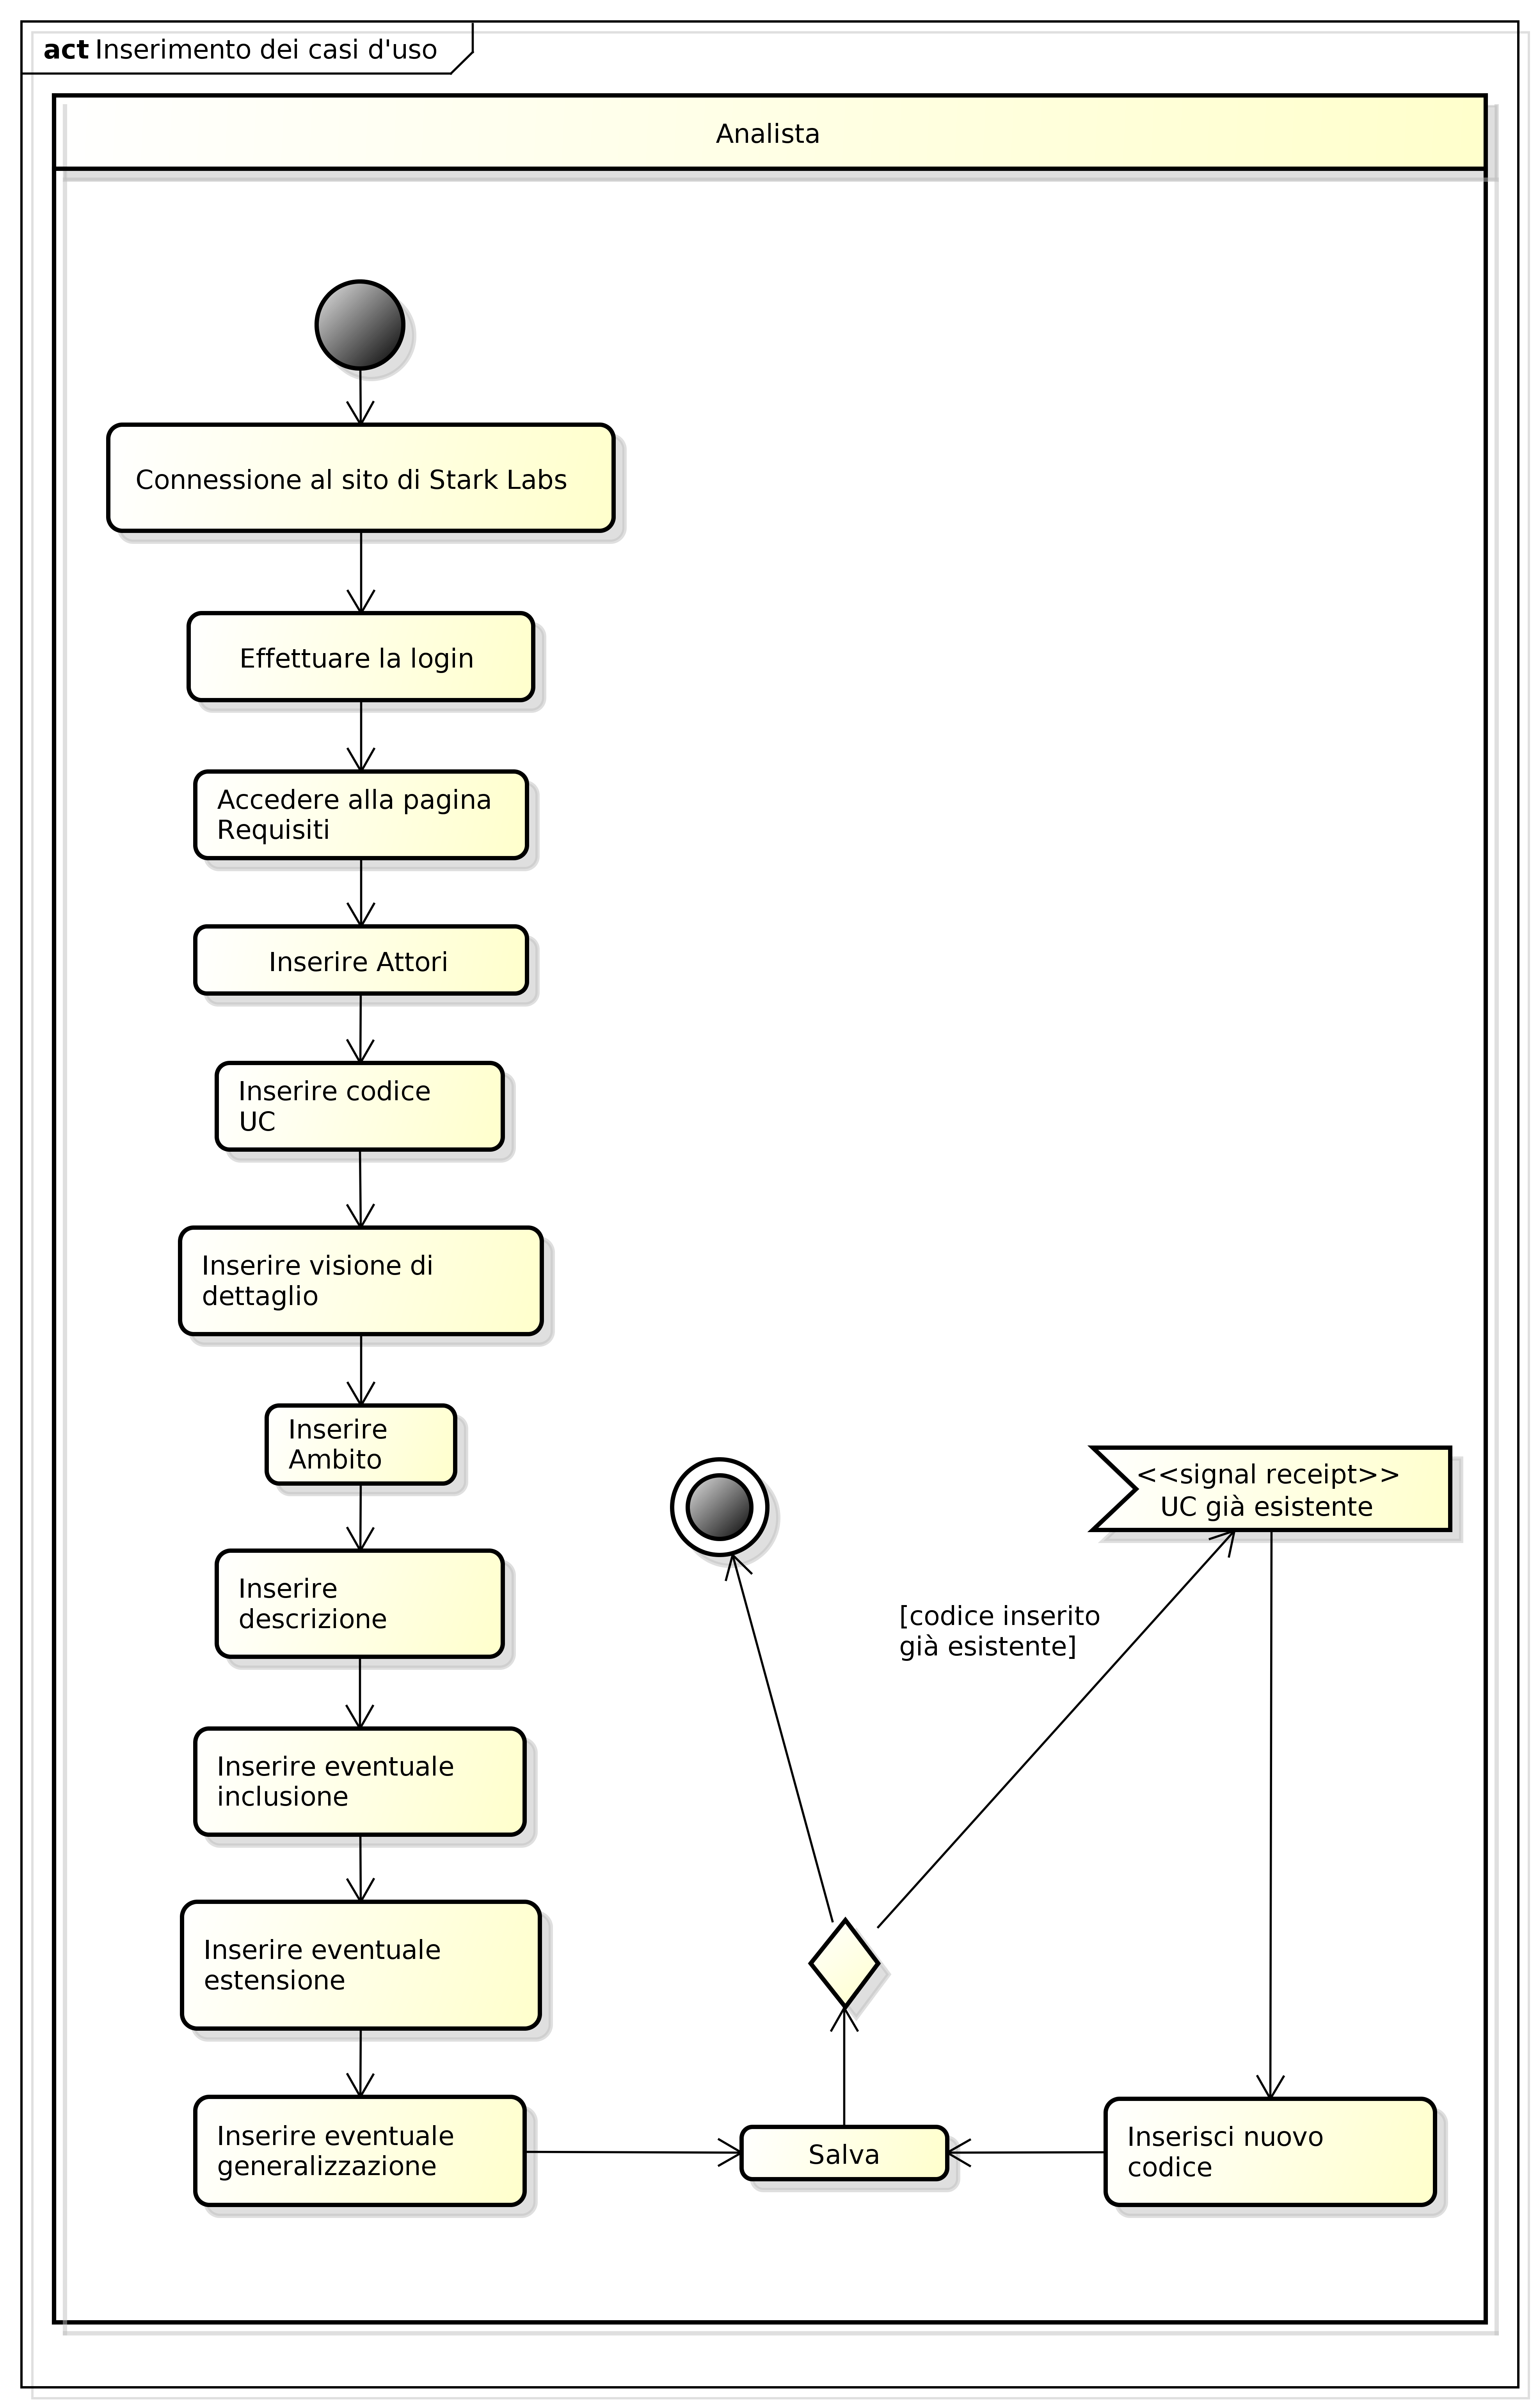
\includegraphics[scale=0.5]{immagini/inserimento_uc.png}
\captionsetup{labelfont=bf}
\caption{Diagramma di attività - Inserimento di un caso d'uso}\label{sec:Figura1}
\end{figure}

\begin{figure}[htbp]
\centering
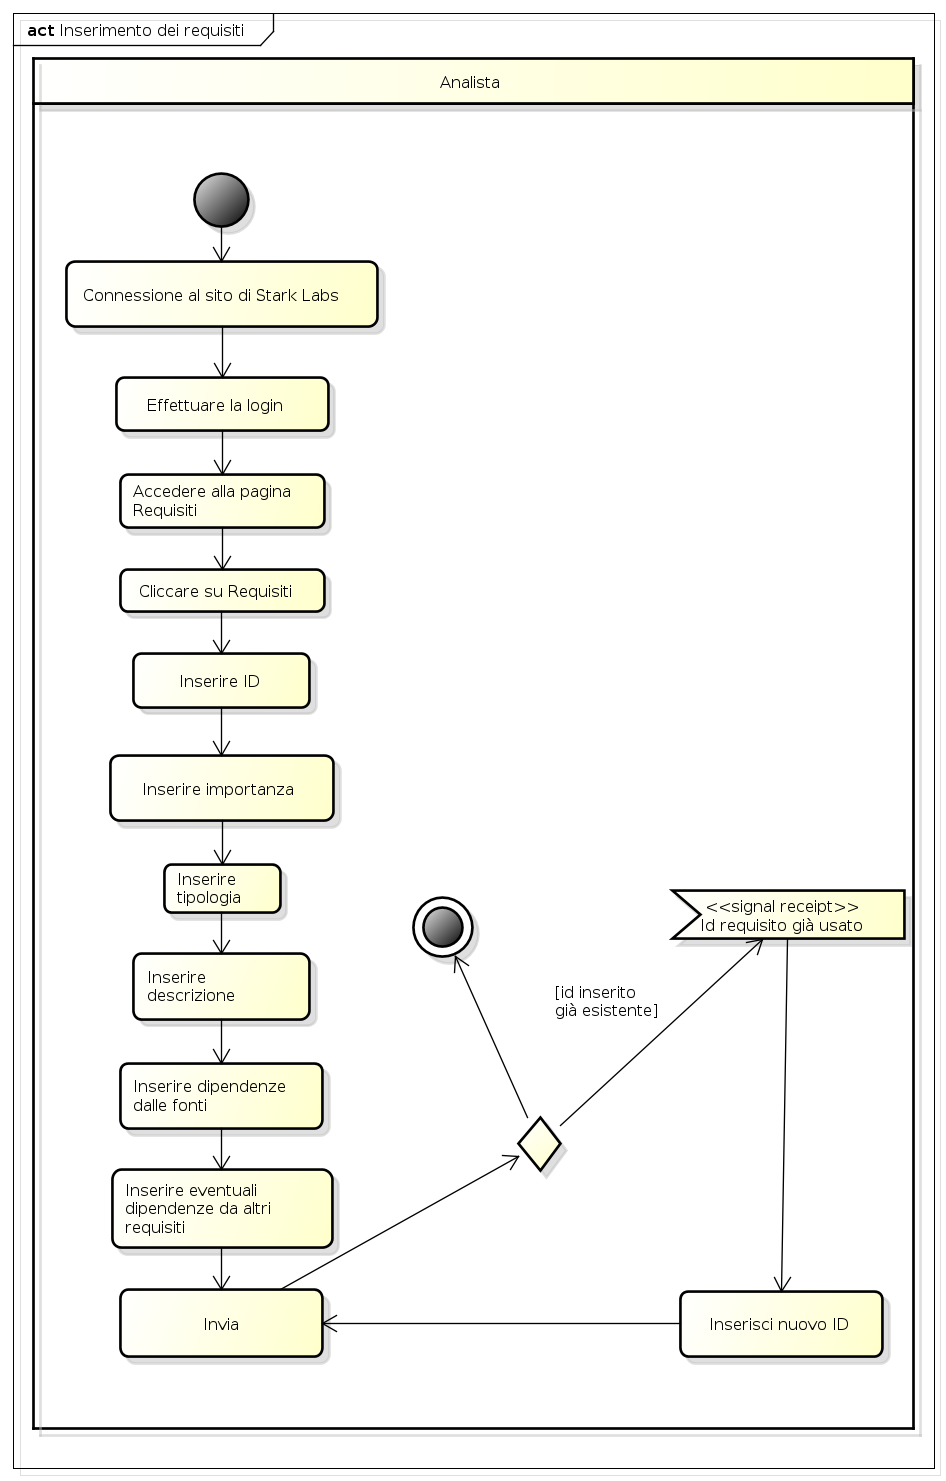
\includegraphics[scale=0.5]{immagini/inserimento_requisiti.png}
\captionsetup{labelfont=bf}
\caption{Diagramma di attività - Inserimento di un requisito}\label{sec:Figura2}
\end{figure}

\newpage

\section{Processi di supporto}
\subsection{Documentazione}
\subsubsection{Attività}
\paragraph{Documentazione} 
Il gruppo di lavoro \GRUPPO\ si impegna a registrare tutte le informazioni acquisite nel corso del ciclo di vita\G\ del \textit{software} all'interno di una serie ben definita di documenti descritti in questa sezione. Nello specifico, vengono spiegati gli standard da rispettare per la stesura dei documenti e i passaggi necessari per renderli formalmente corretti.

\subsubsection{Procedure}
\paragraph{Gestione dei documenti}
La stesura di un nuovo documento viene decisa dal \textit{Responsabile di Progetto}. Tutta la documentazione deve essere creata attraverso l'uso di un \textit{template}\G\ \LaTeX\ disponibile nel \textit{repository}\G\ GitHub\G\ del gruppo, al fine di mantenerne uniforme la struttura e lo stile.

\paragraph{Creazione di un nuovo documento}
Nel \textit{repository}\G\ è presente un \textit{file} generico denonimato \textit{new\_doc.tex} contenente un \textit{template} adattabile ad ogni nuovo documento. Il \textit{file} deve essere incluso con il \textit{template} \LaTeX\, che è messo a disposizione di tutti i membri del gruppo. Ogni redattore deve possedere tutti i \textit{file} previsti dal \textit{template} al fine di creare correttamente un nuovo documento.

\paragraph{Avanzamento di un documento}
La procedura adottata per sviluppare un documento è la seguente ed è riportata in \hyperref[sec:Figura3]{Figura 3}:
\begin{itemize}
	\item [1.] Il \textit{Responsabile di Progetto} si preoccupa di assegnare la stesura del documento a uno o più redattori, a seconda della complessità dello stesso. L'assegnazione è gestita attraverso \textit{task}\G\ organizzati tramite il servizio \textit{online} Teamwork\G; 
	\item [2.] A stesura completata, ogni assegnatario ha il compito di etichettare il \textit{task} come completato;
	\item [3.] Il \textit{Verificatore} riceve in automatico un'email che segnala il completamento del documento;
	\item [4.] Nel caso si riscontrassero errori durante la fase di verifica, il \textit{Verificatore} deve occuparsi di creare un nuovo \textit{task} da assegnare al redattore del documento;
	\item [5.] Nel caso di documento corretto, il \textit{Verificatore} deve completare il \textit{task} assegnatogli. Un'email viene quindi automaticamente recapitata al \textit{Responsabile di Progetto}.
	\item [6.] Il \textit{Responsabile di Progetto} deve infine approvare il documento. In caso di mancata approvazione, il \textit{Verificatore} deve creare un nuovo \textit{task} indirizzato al redattore, che si occuperà di correggere gli errori in base alle segnalazioni emesse. 
\end{itemize}

\begin{figure}[htbp]
\centering
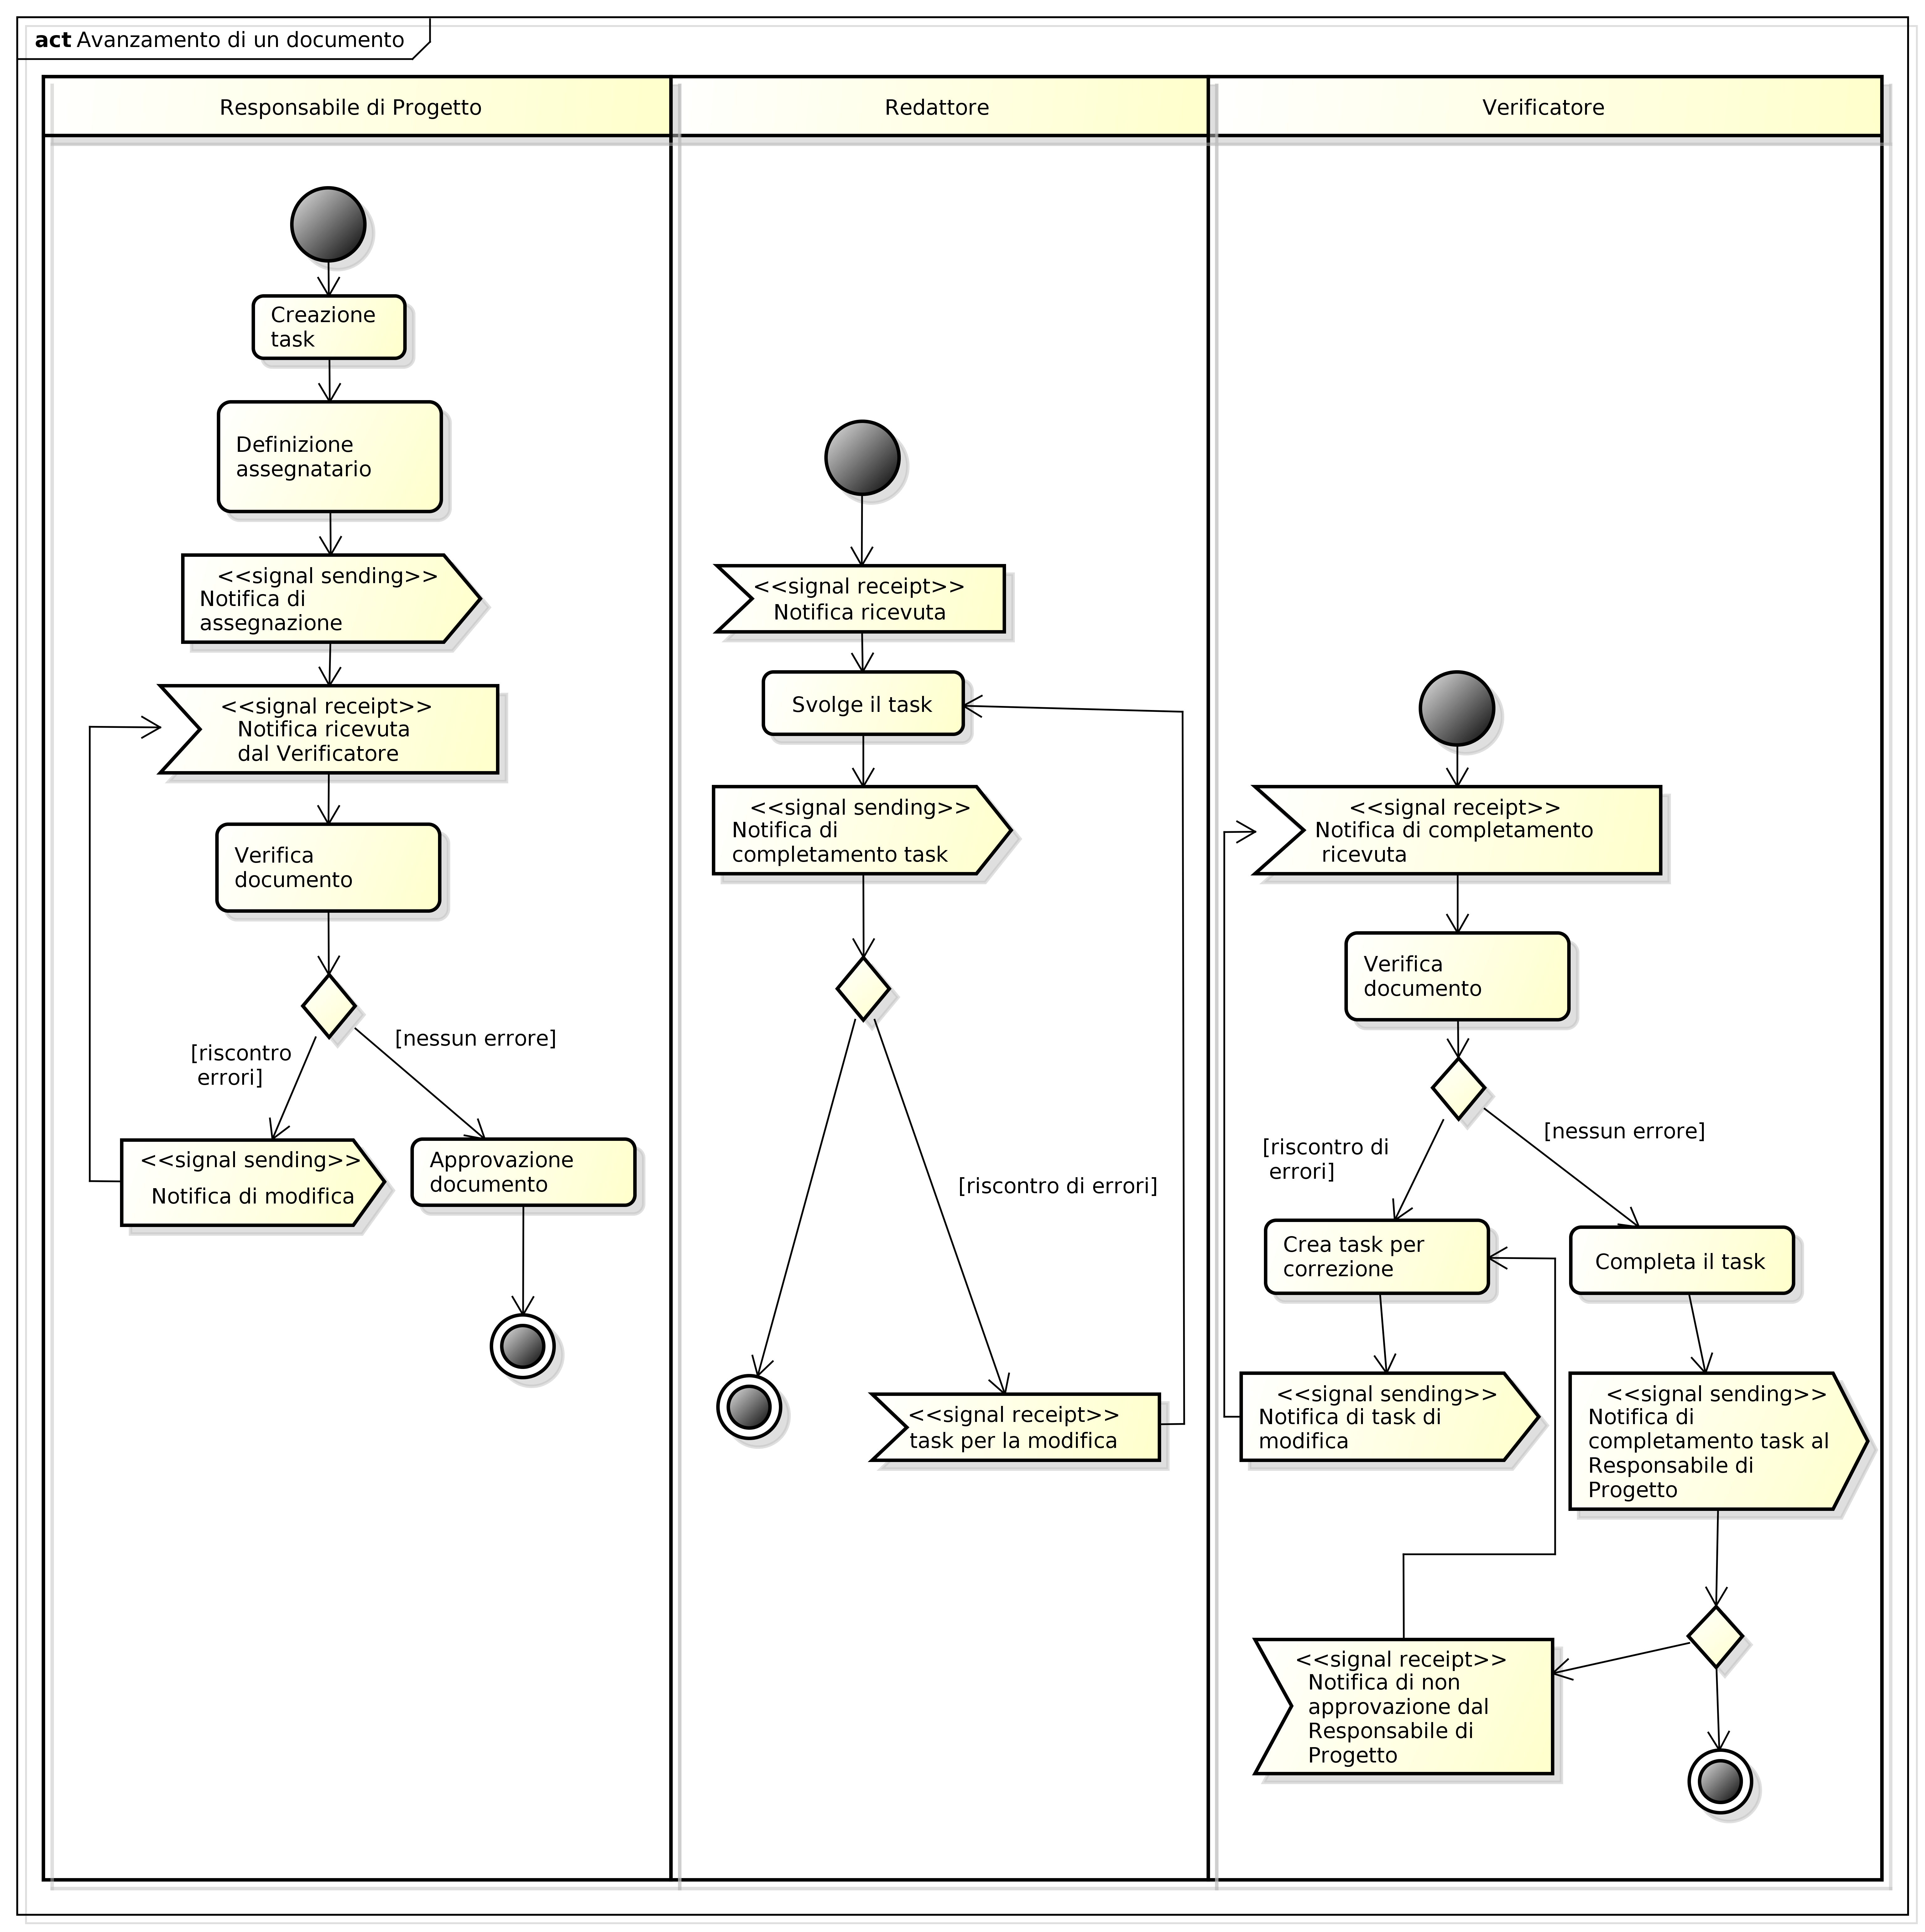
\includegraphics[scale=0.4]{immagini/avanzamento_documento.png}
\captionsetup{labelfont=bf}
\caption{Diagramma di attività - Avanzamento di un documento}\label{sec:Figura3}
\end{figure}

\subsubsection{Gestione del glossario}
Il popolamento del \textit{Glossario v1.0.0} è un'attività, mostrata in \hyperref[sec:Figura4]{Figura 4}, che coinvolge redattori e \textit{Verificatori}, e si svolge come segue:
\begin{itemize}
	\item [1.] {\textbf{Individuazione di un nuovo termine}}: se durante la stesura di un documento il redattore identifica un nuovo termine che ritiene debba essere inserito nel \textit{Glossario v1.0.0}, è tenuto a trascriverlo all'interno di un apposito documento (Glossario Provvisorio) presente nella sezione \textit{Notebooks}\G\ di Teamwork\G.
	\item [2.] {\textbf{Inserimento del termine nel Glossario}}: un \textit{Verificatore} deve occuparsi dell'approvazione di un dato termine presente in Glossario Provvisorio di Teamwork e dell'inserimento dello stesso all'interno del \textit{Glossario v1.0.0}. Una volta inserito, il termine deve essere rimosso dal documento su Teamwork.
\end{itemize}
 Nei documenti, il pedice \G\ appare solamente alla prima occorrenza del vocabolo all'interno di un paragrafo.

\begin{figure}[htbp]
\centering
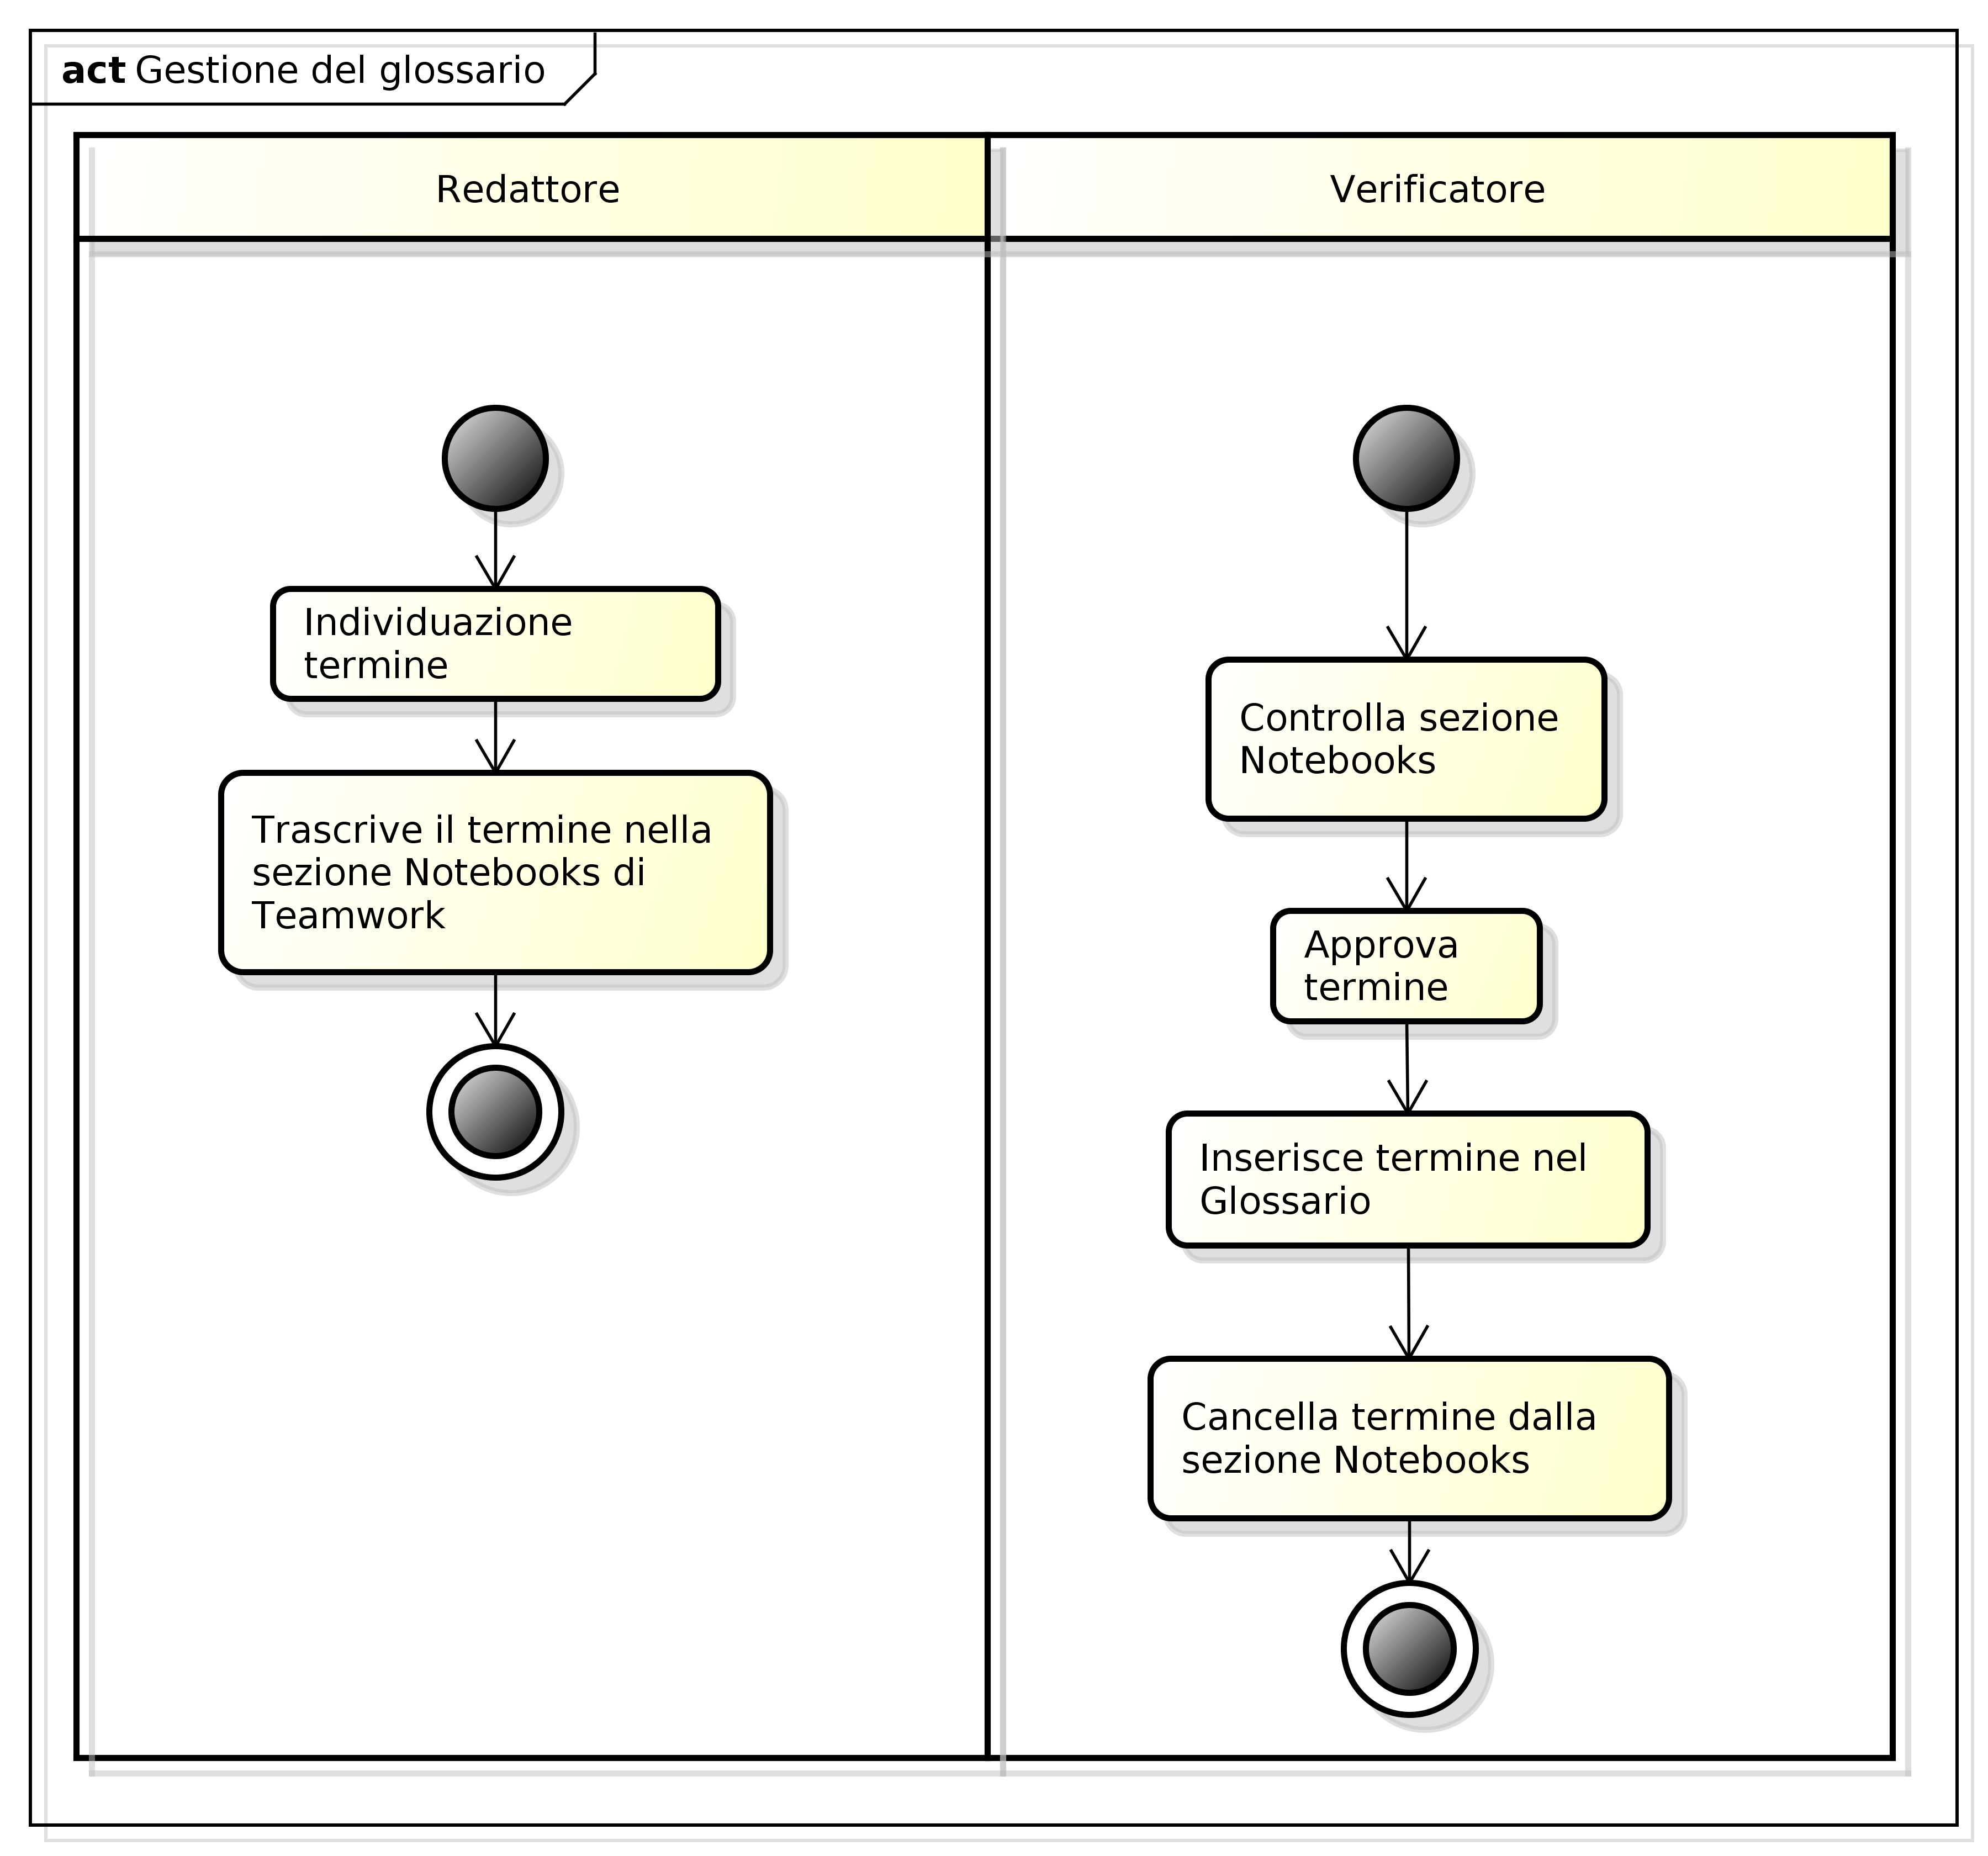
\includegraphics[scale=0.5]{immagini/gestione_glossario.png}
\captionsetup{labelfont=bf}
\caption{Diagramma di attività - Gestione del Glossario}\label{sec:Figura4}
\end{figure}

\subsubsection{Norme}
\paragraph{Progettazione e sviluppo dei documenti}
Ogni documento deve rispettare in modo assoluto la seguente serie di norme.

\paragraph{Versionamento}
\label{sec:versionamento}
Ogni documento prodotto deve essere corredato dal numero di versione. Il formato adottato è
il seguente:
\begin{center}
	vX.Y.Z
\end{center}
tale che:
\begin{itemize}
	\item{\textbf{X}}: indice di versione principale. Tale valore viene incrementato ad ogni approvazione del documento e ne indica la versione di rilascio;
	\item{\textbf{Y}}: indice di modifica parziale. Tale valore viene incrementato ad ogni verifica del documento;
	\item{\textbf{Z}}: indice di modifica minore. Tale valore viene incrementato ad ogni cambiamento che avviene nel documento.
\end{itemize}

\paragraph{Template}
La creazione dei documenti avviene attraverso l'utilizzo di un \textit{template}\G\ sviluppato con \LaTeX\ e la cui struttura \textbf{non} deve essere modificata a meno di direttive imposte dal \textit{Responsabile di Progetto}. Il \textit{template} funge da supporto per la stesura organizzata e sistematica dei documenti e, grazie ad esso, ogni componente del documento ha una precisa impostazione che non può essere modificata o equivocata dai redattori.

\paragraph{Struttura dei documenti}
L'organizzazione dei documenti è la seguente: 
\begin{itemize}
	\item Vi è una cartella generale in cui sono contenuti il \textit{template}\G\ \LaTeX\ e le varie cartelle specifiche di ogni documento;
	\item Nella cartella denominata "\textit{template}" sono contenuti i \textit{file} di configurazione e strutturazione del \textit{template}. Il contenuto della cartella non deve essere modificato, previa autorizzazione da parte del \textit{Responsabile di Progetto};
	\item Nella cartella specifica di ogni documento è presente un \textit{file} di tipo nome\_documento.tex, tramite cui si determina la struttura dello specifico documento. Inoltre è presente una sotto cartella "sezioni" contenente le varie sezioni nelle quali sono scritti i contenuti veri e propri.
\end{itemize}

\subparagraph{Prima pagina}
\label{sec:primaPagina}
Nella prima pagina sono presenti tutte le informazioni generali relative al documento:
\begin{itemize}
	\item Nome del progetto;
	\item Logo del gruppo;
	\item Nome del documento;
	\item Versione del documento;
	\item Membri del gruppo che hanno lavorato come redattori, \textit{Verificatori} e \textit{Responsabili} per la stesura del documento. I nomi vanno scritti nel formato Nome Cognome;
	\item Specifica dell'uso del documento (interno o esterno);
	\item Lista di distribuzione del documento. I nomi vanno scritti nel formato Nome Cognome;
	\item Breve descrizione che precisa lo scopo del documento.
\end{itemize}
\subparagraph{Registro delle modifiche}
Nella seconda pagina si trova una tabella con il registro delle modifiche effettuate al documento. Esso è indispensabile per un corretto tracciamento delle varie fasi che si sono percorse lungo la stesura. Ogni riga corrisponde a una modifica dove vengono segnalati:
\begin{itemize}
	\item Descrizione dell'azione compiuta sul documento;
	\item Nome e cognome dell'autore della modifica;
	\item Data della modifica;
	\item Versione del documento a seguito della modifica.
\end{itemize}

\subparagraph{Indici}
In terza pagina è presente l'indice che tiene traccia delle varie sezioni in cui è stato suddiviso il documento. La profondità dell'indice arriva fino a cinque livelli: gli argomenti trattati sono suddivisi in sezioni, sottosezioni, sotto-sottosezioni, paragrafi e sotto-paragrafi.
Se sono presenti immagini e/o tabelle, viene stilato in automatico un indice che ne tiene traccia.
\subparagraph{Formattazione di una pagina}
Tutte le pagine dei documenti seguono una precisa formattazione imposta dal \textit{template}\G :
\begin{itemize}
	\item{\textbf{Intestazione}}: contiene sulla sinistra il logo del gruppo e sulla destra il nome della sezione in cui è contenuta la pagina;
	\item{\textbf{Contenuto}}: contiene il contenuto effettivo della pagina le cui norme tipografiche sono descritte in \hyperref[sec:normeTipografiche]{3.1.4.5.6 Norme Tipografiche};
	\item{\textbf{Piè di pagina}}: contiene sulla sinistra il nome del documento con relativo numero di versione e sulla destra il numero della pagina, scritto nel formato "X di Y", con X numero di pagina corrente e Y numero delle pagine totali.
\end{itemize}
La suddetta struttura si ripete per ogni pagina ad eccezione della prima, il cui formato è descritto in \hyperref[sec:primaPagina]{3.1.4.4.1 Prima Pagina}.

\paragraph{Suddivisione dei documenti}
\label{sec:suddivisioneDocumenti}
\subparagraph{Norme di Progetto}
Il documento ha lo scopo di definire le linee guida per le varie attività di sviluppo. Al suo interno sono raccolte le norme, le procedure e gli strumenti che il gruppo adotterà nel corso della realizzazione del progetto. Il documento è destinato a uso interno.
\subparagraph{Studio di Fattibilità}
Il documento ha lo scopo di descrivere le considerazioni elaborate dal gruppo per l'accettazione del progetto che si è deciso di prendere in carico, con valutazione di rischi, costi e benefici calcolati sulla base di una prima analisi del capitolato. Al suo interno vengono motivate le scelte che hanno spinto il gruppo all'esclusione degli altri progetti. Il documento è destinato a uso interno.
\subparagraph{Analisi dei Requisiti}
Il documento ha lo scopo di identificare e descrivere i requisiti, i vincoli e gli obiettivi necessari allo sviluppo del progetto. Al suo interno sono contenuti i casi d'uso e i requisiti utili alla realizzazione del progetto, accompagnati da diagrammi e grafici di interazione fra utenti e sistema. Il documento è destinato a uso esterno.
\subparagraph{Piano di Progetto}
Il documento ha lo scopo di pianificare lo svolgimento del progetto. Al suo interno sono fissate le risorse disponibili, la suddivisione e il calendario delle attività, e gli obiettivi necessari per valutare in modo corretto il grado di avanzamento dello sviluppo. Il documento è destinato a uso esterno.
\subparagraph{Piano di Qualifica}
Il documento ha lo scopo di spiegare le strategie applicate al progetto per ottenere gli obiettivi di qualità. Al suo interno sono presenti le attività di verifica e pianificazione con i relativi test da sviluppare. Il documento è destinato a uso esterno.
\subparagraph{Specifica Tecnica}
Il documento ha lo scopo di descrivere l'architettura logica del progetto, senza fissare i dettagli implementativi, ma definendo linee e strategie di realizzazione, al fine di stabilire cause ed effetti e avere una visione complessiva della soluzione. Al suo interno è contenuta una prima progettazione ad alto livello del sistema da sviluppare. In esso vengono specificati i \textit{design pattern}\G\ utilizzati. Il documento è destinato a uso esterno. 
\subparagraph{Definizione di Prodotto}
Il documento ha lo scopo di descrivere nel dettaglio l'architettura del prodotto da sviluppare. Il suo contenuto viene utilizzato dai \textit{Programmatori} per sviluppare il \textit{software}. Il documento è destinato a uso esterno.
\subparagraph{Glossario}
Il documento ha lo scopo di raccogliere, in ordine alfabetico, tutti i termini ambigui presenti nei documenti accompagnati da una loro definizione. Il documento è destinato a uso esterno.

\paragraph{Norme tipografiche}
\label{sec:normeTipografiche}
Al fine di rendere omogenea e coesa la stesura dei documenti, il contenuto deve rispettare le seguenti norme tipografiche.
\subparagraph{Stile del testo}
\begin{itemize}
\item \textbf{Corsivo}: va utilizzato tassativamente per indicare termini in lingua inglese che non fanno parte dell'uso comune dell'italiano, citazioni, nomi di documenti interni, ruoli ufficiali dei membri del gruppo ed eventualmente (ma con moderazione) per parole che si ritiene debbano essere messe in risalto rispetto al resto del testo; 
\item \textbf{Grassetto}: va usato per evidenziare parole significative di estrema importanza. È necessario che non se ne abusi. Viene applicato automaticamente a titoli di sezioni, sottosezioni e paragrafi. Viene utilizzato negli elenchi puntati per evidenziare un termine seguito da una descrizione;
\item \textbf{Maiuscolo}: viene utilizzato per scrivere acronimi e macro \LaTeX. Inoltre, lettere maiuscole vengono usate per riferirsi ai ruoli di progetto, alle fasi di lavoro e ai seguenti nomi: del \textit{team}, del progetto e dei documenti;
\item \LaTeX: viene usato il comando \textbackslash LaTeX per ogni occorrenza del termine \LaTeX;
\item \textbf{Font}: nel \textit{template} è impostato Gillius, un \textit{font} professionale di tipo \textit{sans-serif} il cui scopo è garantire maggiore leggibilità del testo su schermo;
\item \textbf{Monospace}\G: tipologia di font che serve per formattare correttamente il testo contenente porzioni di codice, comandi e indirizzi \textit{web}.
\end{itemize}
\subparagraph{Punteggiatura}
\begin{itemize}
\item \textbf{Spaziatura}: lo spazio non può mai precedere un carattere di punteggiatura.
\end{itemize} 
\subparagraph{Composizione del testo}
\begin{itemize}
	\item {\textbf{Elenchi puntati}}: l’ultima voce deve terminare con un punto, mentre le altre con un punto e virgola. La prima lettera di ogni punto va scritta in maiuscolo e la prima parola va in grassetto se seguita da una descrizione della stessa. Gli elenchi numerati vengono utilizzati per descrivere sequenze di azioni ordinate;
	\item \textbf{Pedice G}: il pedice \G\ è utilizzato al solo scopo di indicare termini potenzialmente ambigui che si possono reperire nel documento \textit{Glossario v1.0.0}.
\end{itemize}

\subparagraph{Formati} Elenco dei formati rispettati dai documenti:
\begin{itemize}
	\item \textbf{Data}: il formato utilizzato è dd/mm/yyyy. Per esempio, 16/11/2004 indica il 16 novembre 2004;
	\item \textbf{Ora}: si utilizza il formato internazionale previsto dalla norma ISO 8601 del tipo [hh]:[mm]:[ss] ove [hh] indica l'ora, [mm] i minuti, [ss] i secondi, espressi con due cifre. Ad esempio, 18:35:26 indica le ore 18, 35 minuti e 26 secondi; 04:09:01 indica le ore 4, 9 minuti e 1 secondo;
	\item \textbf{Percorsi}: viene utilizzato il separatore \textit{slash} (/) per indicare il percorso di un \textit{file}. Per esempio, cartella1/cartella2/file\_esempio.txt;
	\item \textbf{Nomi di persona}: espressi nel formato Nome Cognome.
\end{itemize}

\subparagraph{Sigle} Elenco delle sigle che possono apparire nel corso dei documenti:
\begin{itemize}
	\item \textbf{AdR}: Analisi dei Requisti; 
	\item \textbf{GL}: Glossario; 
	\item \textbf{NdP}: Norme di Progetto; 
	\item \textbf{PdP}: Piano di Progetto;
	\item \textbf{PdQ}: Piano di Qualifica; 
	\item \textbf{SdF}: Studio di Fattibilità;
	\item \textbf{ST}: Specifica Tecnica; 
	\item \textbf{RA}: Revisione di Accettazione;
	\item \textbf{RP}: Revisione di Progettazione;
	\item \textbf{RQ}: Revisione di Qualifica;
	\item \textbf{RR}: Revisione dei Requisiti.
\end{itemize}

\paragraph{Componenti grafiche}
\subparagraph{Immagini e diagrammi}
Tutte le immagini (diagrammi inclusi) da inserire nei documenti devono essere salvate in formato \textit{Portable Network Graphics} (PNG\G) o \textit{Portable Document Format} (PDF\G). Immagini e diagrammi vanno inserite nella cartella "immagini" relativa al documento specifico.

\subsection{Processo di verifica e validazione}
Il processo di verifica consiste nel controllare che il materiale prodotto al raggiungimento delle \textit{milestone}\G\ sia conforme agli obiettivi prefissati. Pertanto, è necessario verificare che non siano stati commessi errori. Il prodotto è validato se il risultato ottenuto è consistente e conforme alle attese. Una corretta applicazione del processo di verifica genera un aumento del rapporto fra efficienza ed efficacia, riducendo il tempo impiegato nel percorso di analisi e correzione.
\subsubsection{Attività}
\paragraph{Analisi statica}
L'attività di analisi statica è una tecnica di verifica applicabile sia a documenti che a codice sorgente che va ad analizzare il solo testo del \textit{file} senza mandarlo in esecuzione. Tale tecnica viene utilizzata durante l'intero sviluppo del progetto e si pone come obiettivo il ritrovamento di eventuali anomalie. I metodi di controllo sono i seguenti:
\begin{itemize}
	\item \textbf{Walktrough}: si ricercano all'interno di testo o codice tutte le possibili anomalie; l'attività è eseguita da persone. L'analisi si basa sulla lettura di tutto il contenuto del \textit{file}. In seguito al ritrovamento di anomalie, le si analizza con il redattore del documento (o \textit{Programmatore} nel caso di codice) e si indaga per raggiungere una soluzione del problema. Tale tecnica risulta utile durante le prime fasi di sviluppo del progetto, in quanto manca, ai componenti, una visione complessiva del documento o del codice che si sta scrivendo. Permette così ai \textit{Verificatori}, dopo aver svolto le prime correzioni, di preparare una \textit{lista di controllo} con gli errori più frequenti in modo da migliorare l'efficienza delle verifiche future. A questo punto è possibile implementare un'analisi mirata e più efficiente attraverso il metodo dell'\textit{Inspection}.
	\item \textbf{Inspection}: si ricercano all'interno di un testo errori specifici; l'attività può essere eseguita sia da un umano che, nel caso di anomalie nella sintassi, da uno script. Il metodo focalizza la ricerca su errori presupposti identificati dalla \textit{lista di controllo}.
\end{itemize}
\paragraph{Analisi dinamica}
L'attività di analisi dinamica è una tecnica di verifica applicabile solamente al \textit{software}. Tale tecnica può essere utilizzata per analizzare l'intero \textit{software} o una porzione limitata dello stesso. L'attività consiste nell'esecuzione di \textit{test} automatici realizzati dal \textit{team}. Le verifiche devono essere effettuate su un insieme finito di casi, con valori di ingresso, uno stato iniziale e un esito decidibile. Tutti i \textit{test} producono risultati automatici che inviano notifiche sulla tipologia di problema individuato. Ogni \textit{test} è ripetibile, ossia applicabile durante l'intero ciclo di vita\G\ del \textit{software}. Le caratteristiche da rispettare sono le seguenti: 
\begin{itemize}
	\item \textbf{Ambiente}: è necessario riportare l'ambiente sia \textit{software} che \textit{hardware} in cui il sistema esegue il \textit{test}. Deve essere specificato lo stato iniziale del sistema; 
	\item \textbf{Specifica}: è necessario riportare i dati in ingresso e in uscita per verificare l'esito del \textit{test}, ossia se il codice analizzato è conforme alle aspettative;
	\item \textbf{Procedure}: è possibile specificare ulteriori istruzioni per l'esecuzione dei \textit{test}. Inoltre possono essere riportate istruzioni sulla corretta lettura dei risultati.
\end{itemize}
\paragraph{Gestione anomalie}
Se si dovessero riscontrare anomalie o discordanze normative durante le attività di verifica, il \textit{Verificatore} ha il dovere di notificarle all'assegnatario del \textit{task}\G.  

\paragraph{Tracciamento}
L'attività di tracciamento svolta dai \textit{Verificatori} consiste nella catalogazione di tutti i casi d'uso e dei requisiti che ne derivano ed evidenziare la corrispondenza fra di essi in modo da avere ben chiaro i processi di derivazione.

\subsubsection{Procedure}
\paragraph{Procedure di assegnazione delle anomalie}
L'assegnazione delle anomalie rilevate dai \textit{Verificatori} avviene attraverso l'uso del servizio \textit{web} Teamwork\G. Gli errori vanno gestiti attraverso \textit{task}\G\ da creare in una delle seguenti categorie:
\begin{itemize}
	\item \textbf{Anomalie Documenti}: gruppo di \textit{task} dedicato agli errori rilevati nella documentazione;
	\item \textbf{Anomalie Codice}: gruppo di \textit{task} dedicato agli errori rilevati nel codice.
\end{itemize}
I \textit{task} contenuti nei suddetti gruppi devono essere creati seguendo la seguente serie di azioni, mostrate anche in \hyperref[sec:Figura5]{Figura 5}:
\begin{itemize}
	\item [1.] Assegnazione di un titolo al nuovo \textit{task} contenente in testa la dicitura [BUG];
	\item [2.] Descrizione dettagliata dell'anomalia rilevata. Deve essere specificato il punto esatto del file in cui è stato individuato l'errore;
	\item [3.] Assegnazione del \textit{task} al membro del gruppo che ha commesso l'errore;
	\item [4.] Assegnazione di una data di scadenza per la correzione dell'errore.
\end{itemize} 
Una volta creato il \textit{task}, un'email viene inviata automatica all'assegnatario, che avrà l'incarico di risolvere il \textit{bug}\G\ entro la data di scadenza segnata. La priorità di risoluzione degli errori deve essere svolta secondo l'ordine di scadenza organizzato dal \textit{Responsabile di Progetto}.

\begin{figure}[htbp]
\centering
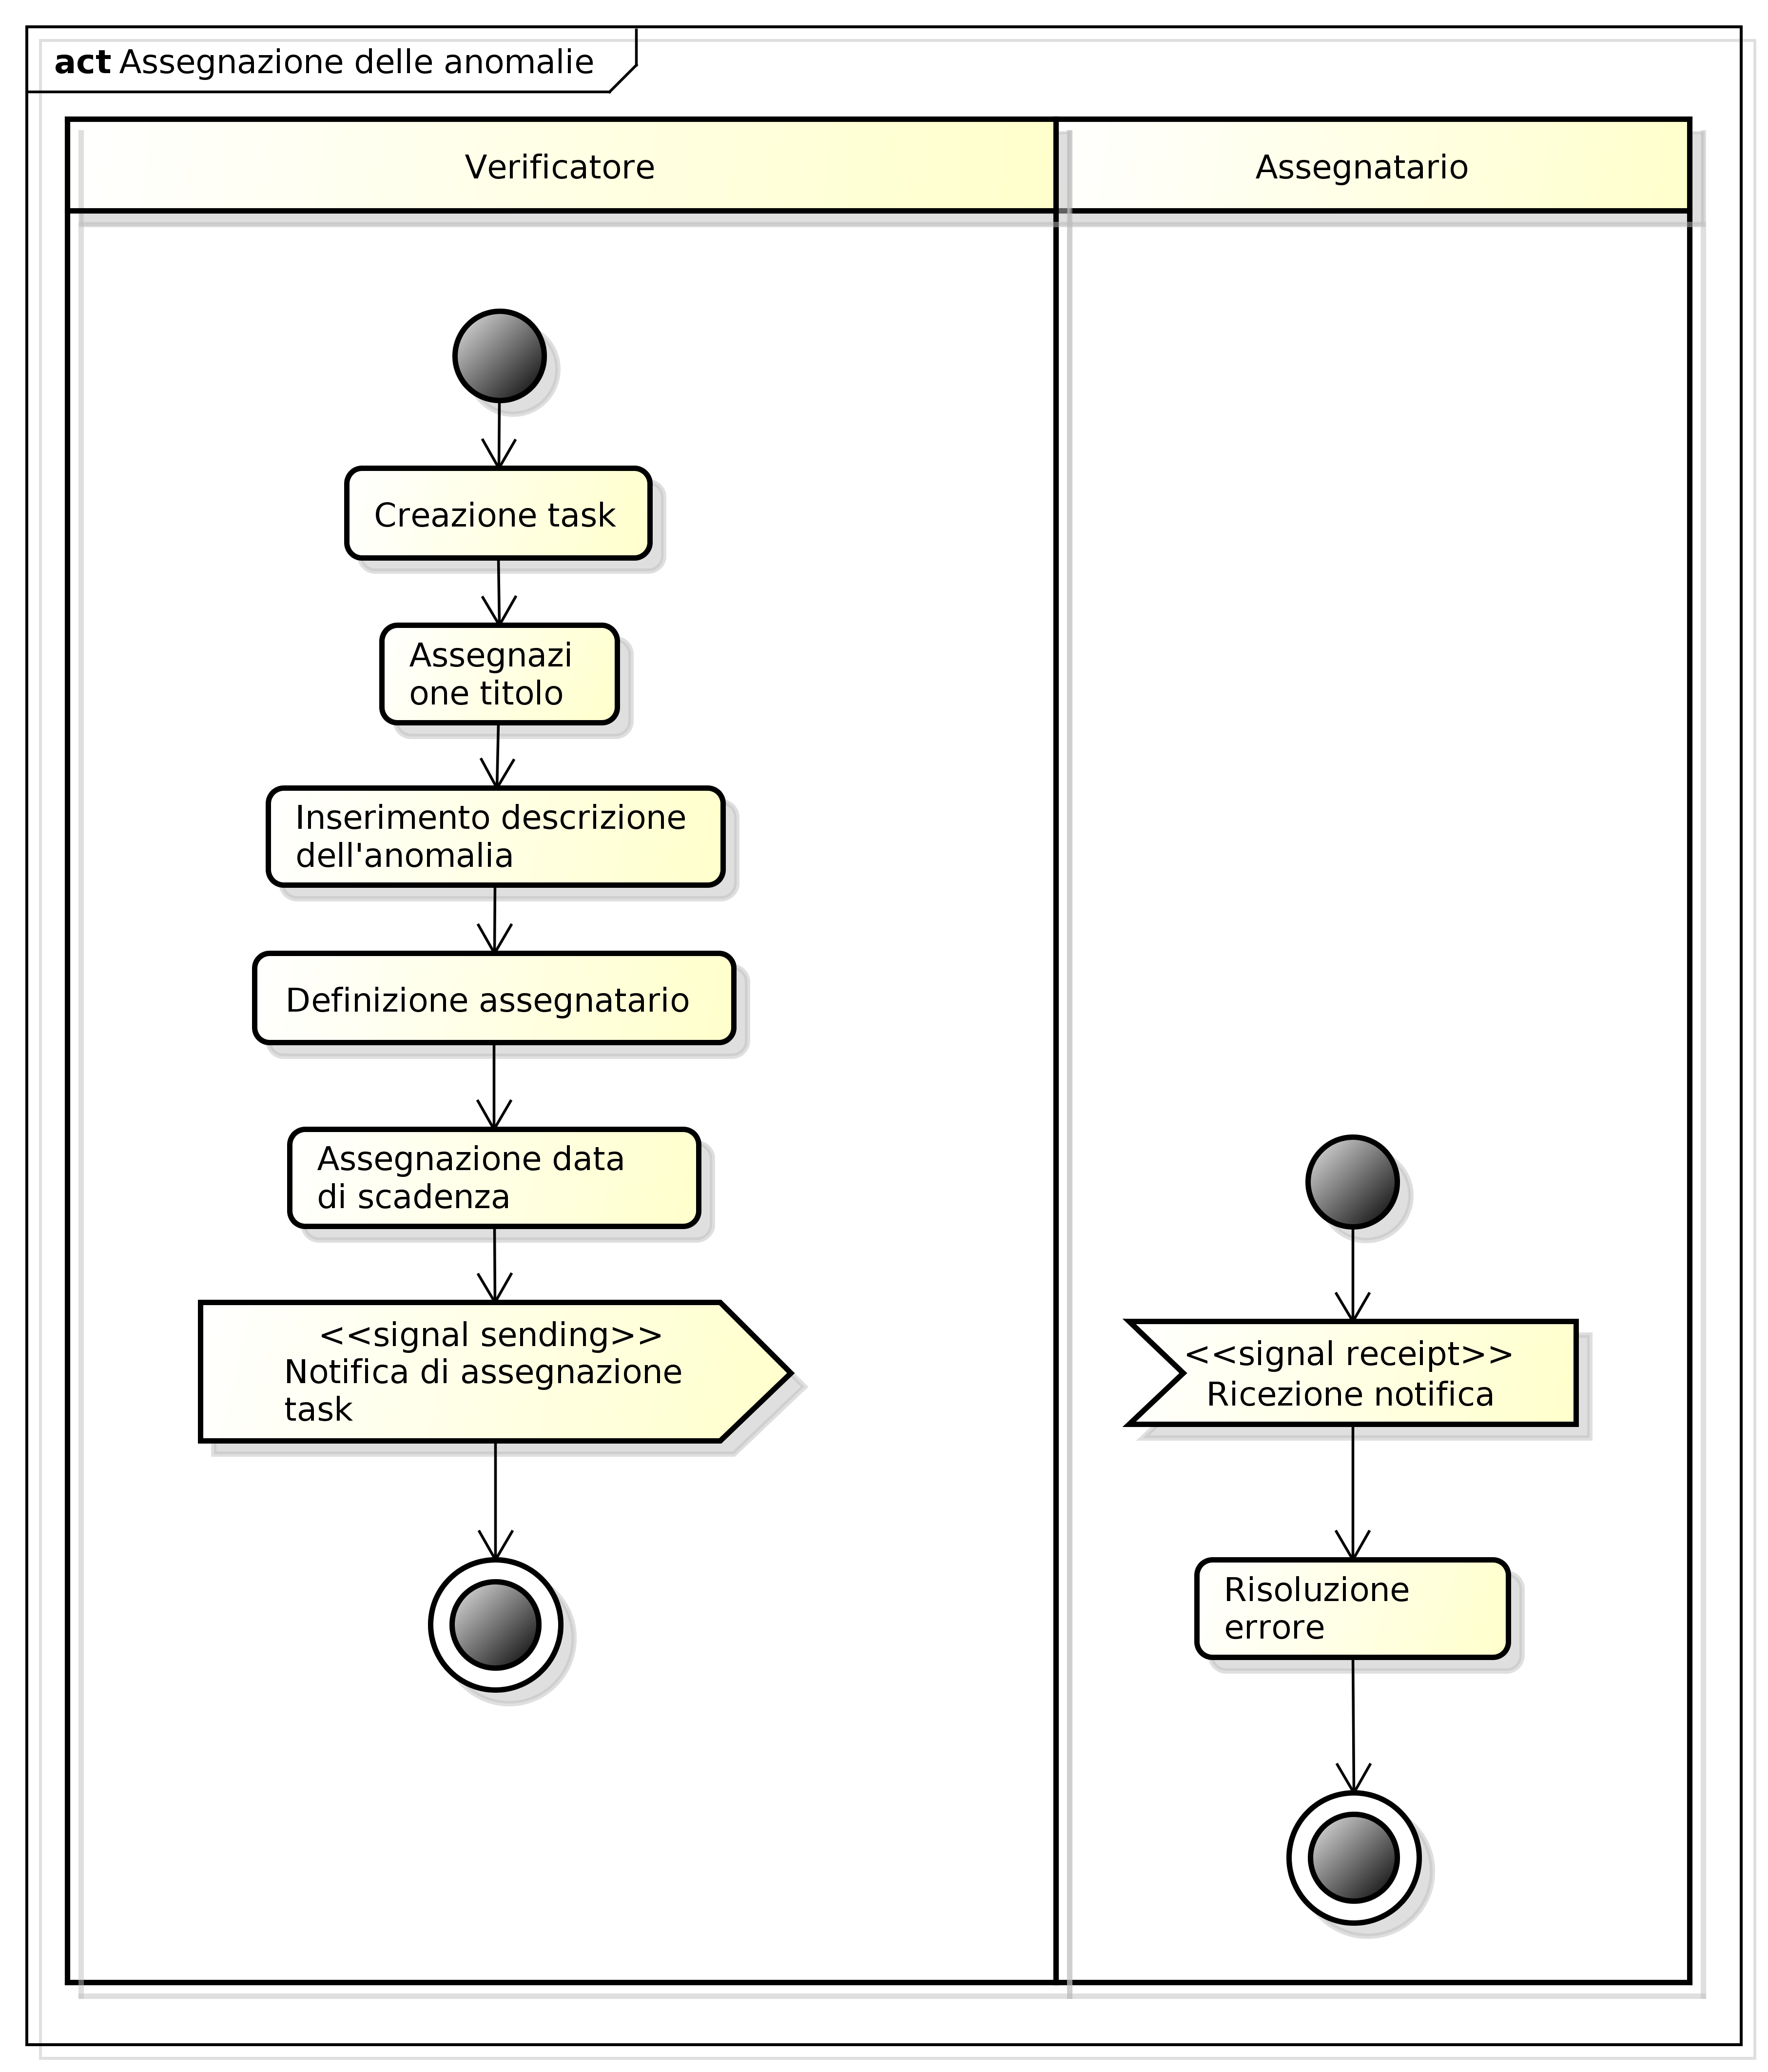
\includegraphics[scale=0.5]{immagini/assegnazione_anomalie.png}
\captionsetup{labelfont=bf}
\caption{Diagramma di attività - Procedura di assegnazione delle anomalie}\label{sec:Figura5}
\end{figure}

\subsubsection{Strumenti}
\paragraph{Correzione ortografica}
Come supporto alla correzione dei documenti si utilizza il correttore ortografico automatico incluso nell'\textit{editor} TeXstudio\G. Gli strumenti offerti da TeXstudio sono utili alla sola correzione di errori ortografici gravi, ma non è preciso per l'individuazione di errori più sottili. Un'analisi più approfondita spetta ai \textit{Verificatori}.
\paragraph{Calcolo dell'indice Gulpease}
Affinchè un documento possa superare la fase di accettazione, è necessario che soddisfi il test di leggibilità con un indice Gulpease\G\ superiore a 40 punti. Per maggiori dettagli si veda il documento \textit{Piano di Qualifica v1.0.0}.
\newpage
\section{Processi organizzativi}
\subsection{Gestione dei processi}
\subsubsection{Attività}
\paragraph{Gestione delle comunicazioni}
\subparagraph{Comunicazione interna}
Viene utilizzato un gruppo Telegram\G\ per comunicare informalmente fra i membri del \textit{team}.
Il servizio fornisce il vantaggio di essere un'applicazione 
multipiattaforma\G\ e disponibile nelle versioni \textit{desktop}, \textit{web} e \textit{mobile}. Inoltre è possibile catalogare e tenere traccia degli argomenti tramite l'uso di \textit{hashtag}\G\ (per esempio: \#analisiRequisiti), e chiamare all'attenzione un dato membro attraverso l'utilizzo del comando chiocciola (per esempio: @GordonFreeman).

\subparagraph{Comunicazione esterna}
Il \textit{Responsabile di Progetto} è la persona preposta a mantenere i contatti con 
individui esterni al gruppo. Per tali comunicazioni è stato creato il 
seguente indirizzo di posta elettronica:
\begin{center}
	starklabs.swe@gmail.com
\end{center}
Tutti i componenti del gruppo possono accedere all'indirizzo di posta, tuttavia solo 
il \textit{Responsabile di Progetto} può inviare comunicazioni con tale indirizzo email. 
Tutte le email ricevute verranno automaticamente inoltrate agli indirizzi personali dei membri del \textit{team}.

\subparagraph{Composizione email}
\begin{itemize}
\item \textbf{Destinatario:}
\begin{itemize}
\item I destinatari possono essere il Proponente (Giulio Paci e l'azienda MIVOQ s.r.l.), il Prof. Tullio Vardanega e il Prof. Riccardo Cardin.
\end{itemize}
\item \textbf{Mittente:}
\begin{itemize}
\item L'unico indirizzo utilizzabile è starklabs.swe@gmail.com e può essere usato solamente dal \textit{Responsabile di Progetto}.
\end{itemize}

\item \textbf{Oggetto:} l'oggetto deve contenere la dicitura [UNIPD-TTS] così come è stato specificato nel capitolato dell'azienda Proponente. Nel caso il messaggio sia una risposta è consigliabile aggiungere la particella “Re:” all'inizio dell'oggetto per rendere chiara la distinzione del livello di risposta; se si dovesse trattare di un inoltro si deve usare la particella “I:”. L'oggetto non va mai cambiato.

\item \textbf{Corpo:} in caso di risposta da parte dell'azienda MIVOQ o del Committente,
risulta utile la citazione della frase a cui si intende rispondere. Il modello per citare correttamente una porzione del messaggio deve rispettare le seguenti regole: devono essere presenti data e ora della mail a cui si risponde, il nome del mittente e il suo 
indirizzo email tra parentesi angolari. Per esempio: <starklabs.swe@gmail.com>, 
la dicitura “ha scritto:” e infine il testo con all'inizio una parentesi angolare chiusa (“>testo di prova”). 
Se dovessero essere presenti alcune parti con uno o 
più destinatari specifici, il nome dovrà essere indicato all'inizio del paragrafo attraverso la dicitura: \textit{@destinatario}.

\item \textbf{Allegati:} qualora vi fosse necessità, è possibile allegare alcuni \textit{file} al 
messaggio email. Possono per esempio essere allegati i verbali di eventuali incontri con 
Proponente o Committente, oppure \textit{file} facenti parte della documentazione spiegata in sezione \hyperref[sec:suddivisioneDocumenti]{3.1.4.5 Suddivisione dei documenti}.
\end{itemize}


\paragraph{Gestione delle riunioni}
\subparagraph{Riunioni interne}
\begin{itemize}
\item \textbf{Frequenza:} le riunioni del gruppo di lavoro avranno cadenza settimanale; 

\item \textbf{Convocazione:} Il \textit{Responsabile di Progetto} ha il compito di convocare le riunioni generali, a 
cui dovranno partecipare tutti i membri del gruppo.
Su decisione del \textit{Responsabile di Progetto} le riunioni possono coinvolgere anche 
solo specifici componenti del gruppo, a seconda del ruolo che si ritiene più 
utile in una data fase del progetto. Al termine di ogni riunione viene redatto 
un verbale.
Il \textit{Responsabile} deve convocare l'assemblea con almeno un giorno di preavviso
attraverso l'invio di una comunicazione ufficiale nel gruppo Telegram\G, messa in rilievo tramite l'uso dell'\textit{hashtag}\G\ \#riunioneDATA, 
con DATA espressa nel formato d/mmmm/yyyy. Per esempio: \#riunione8marzo2016 raccoglie i messaggi inerenti alla riunione tenutasi in data 8 marzo 2016. Nel corpo del messaggio deve essere specificato:
\begin{itemize}
	\item \textbf{Data}: data e ora prevista;
	\item \textbf{Luogo}: luogo previsto;
	\item \textbf{Tipo}: ordinaria o straordinaria;
	\item \textbf{Ordine del giorno}: elenco ordinato delle voci da esaminare.
\end{itemize}

Ogni componente del gruppo deve rispondere al messaggio nel più breve tempo possibile, confermando la presenza o giustificando l'eventuale assenza. In assenza di una risposta di uno o più membri entro 24 ore, il \textit{Responsabile di Progetto} ha il compito di contattare telefonicamente gli interessati. Una volta ricevute le 
risposte e verificata l'assenza o presenza dei membri convocati, il 
\textit{Responsabile di Progetto} ha la possibilità di decidere se confermare o 
posticipare la riunione, in modo da permettere la presenza di tutti i membri chiamati; 
tutte le eventuali modifiche dovranno essere notificate tramite lo stesso \textit{hashtag} utilizzato per organizzare la riunione. 

\item \textbf{Verbale:} il verbale di riunione interna si presenta in forma di documento 
informale, utile al solo scopo di fissare in modo ordinato i punti principali trattati e le relative soluzioni proposte. Il verbale deve essere redatto come documento testuale utilizzando la funzione \textit{Notebooks}\G\ di Teamwork\G. In questo modo si facilita la condivisione, tra tutti i membri del gruppo, di un documento mantenuto aggiornato dal segretario della riunione. Tale ruolo viene scelto a rotazione tra i membri convocati. È inoltre compito del segretario annotare ogni argomento trattato e controllare che venga rispettato l'ordine del giorno.

\end{itemize}

\subparagraph{Riunioni esterne}
\begin{itemize}
\item \textbf{Convocazione}: in questo caso viene utilizzata l'email starklabs.swe@gmail.com attraverso la quale il \textit{Responsabile di Progetto} si occupa di contattare l'azienda Proponente e di mettere in cc\G\ i membri del gruppo. Per quanto sia auspicabile una riunione plenaria, eventuali assenze 
dei componenti del \textit{team} non causeranno posticipazioni o spostamenti delle 
date di incontro, dovendo ovviamente considerare gli impegni dell'azienda stessa.

\item \textbf{Verbale}: in caso di riunione con il Committente o il Proponente, il verbale è un 
documento che assume carattere ufficiale e che pertanto viene redatto secondo uno schema 
specifico.
Per agevolare la scrittura di tale documento viene utilizzato un \textit{template}\G\ 
\LaTeX\ per definire la struttura e organizzare i contenuti. Tale documento 
dovrà essere redatto e inviato come allegato in risposta all'email di convocazione 
dell'assemblea al Proponente Giulio Paci direttamente dal segretario scelto tra i membri presenti. 
\end{itemize}


\paragraph{Gestione del sistema dei task} Il sistema selezionato per la gestione dei \textit{task}\G\ è Teamwork\G, un servizio \textit{web} di \textit{project management}\G. Le viste presenti sono:
\begin{itemize}
\item \textbf{Dashboard}: dove vengono visualizzati i progetti attivi e le ultime notizie relative ad essi;

\item \textbf{Everything}: che consente di visualizzare i \textit{task}, le \textit{milestone}\G\ e i \textit{file} con possibilità di filtrarli per data;

\item \textbf{Project}: permette di visualizzare la lista di tutti i progetti suddivisi per categoria e ne consente l'accesso;

\item \textbf{Calendar}: mostra un calendario per la gestione degli impegni e delle scadenze;

\item \textbf{Statuses}: consente di verificare gli stati dei collaboratori del progetto;

\item \textbf{People}: permette di visualizzare l'elenco dei singoli elementi del gruppo di lavoro e di accedere al loro profilo.    
\end{itemize}

Le funzionalità principali si hanno in seguito all'accesso al progetto desiderato. Esse si suddividono nei seguenti punti:
\begin{itemize}
\item Aggiunta di nuovi \textit{task}, ed eventualmente di sotto \textit{task}, da associare ad uno o più membri del \textit{team};

\item Assegnazione a ciascun \textit{task}\ di una data d'inizio e di completamento;

\item Aggiunta di nuove \textit{milestone}\ con relativi dettagli come responsabile, descrizione e data di scadenza;

\item \textit{Upload}\G\ di file potenzialmente utili al gruppo di lavoro;

\item Utilizzo di un blocco note.
 
\end{itemize}

\paragraph{Gestione delle milestone} 
Il \textit{Responsabile di Progetto} ha il compito di pianificare i punti di controllo che il \textit{team} deve raggiungere, assicurandosi che ogni \textit{task}\G\ necessario al suo soddisfacimento venga terminato entro la data prestabilita.

\paragraph{Gestione dei task} 
È compito del \textit{Responsabile di Progetto} individuare ogni singolo \textit{task}\G\ e, al seguito di un'accurata valutazione, assegnarlo al membro del gruppo più adatto. Deve inoltre associare una data di inizio e di scadenza di fattibilità. Tutte queste attività possono essere facilmente accedute attraverso l'interfaccia grafica di Teamwork\G.

\paragraph{Gestione dello svolgimento dei task}
Ogni membro del gruppo di lavoro è tenuto ad accettare il \textit{task}\G\ assegnatogli dal \textit{Responsabile di Progetto} e fare quanto possibile per portarlo a termine entro la data di scadenza. Nel caso in cui l'assegnatario non fosse in grado di adempire al suo compito è tenuto a renderlo noto al \textit{Responsabile di Progetto} entro 24 ore dall'assegnazione del \textit{task}, altrimenti quest'ultimo verrà considerato come accettato; solo dopo un'accurata valutazione delle motivazioni riportate, il \textit{Responsabile di Progetto} può provvedere a trovare un nuovo membro da incaricare allo svolgimento del \textit{task}.

\subsubsection{Procedure}
\paragraph{Generazione di una milestone}
Dopo aver avuto accesso al progetto di Teamwork\G, il \textit{Responsabile di Progetto} deve eseguire i seguenti passi per generare una \textit{milestone}\G:
\begin{itemize}
\item [1.] Cliccare sul pulsante \textit{"Add a milestone"};
\item [2.] Definire il titolo della \textit{milestone};
\item [3.] Definire la data di scadenza;
\item [4.] Assegnarla ad un responsabile.
\end{itemize}

\paragraph{Assegnazione di un task}
Dopo essere acceduto al progetto di Teamwork\G, il \textit{Responsabile di Progetto} deve eseguire i seguenti passi, mostrati anche in \hyperref[sec:Figura6]{Figura 6}, per generare un \textit{task}\G\:
\begin{itemize}
\item [1.] Cliccare sul pulsante \textit{"Add a task"};
\item [2.] Definire il titolo del \textit{task};
\item [3.] Definire la data di inizio;
\item [4.] Definire la data di scadenza;
\item [5.] Assegnarlo ad uno o più membri del gruppo.
\end{itemize}

\begin{figure}[htbp]
\centering
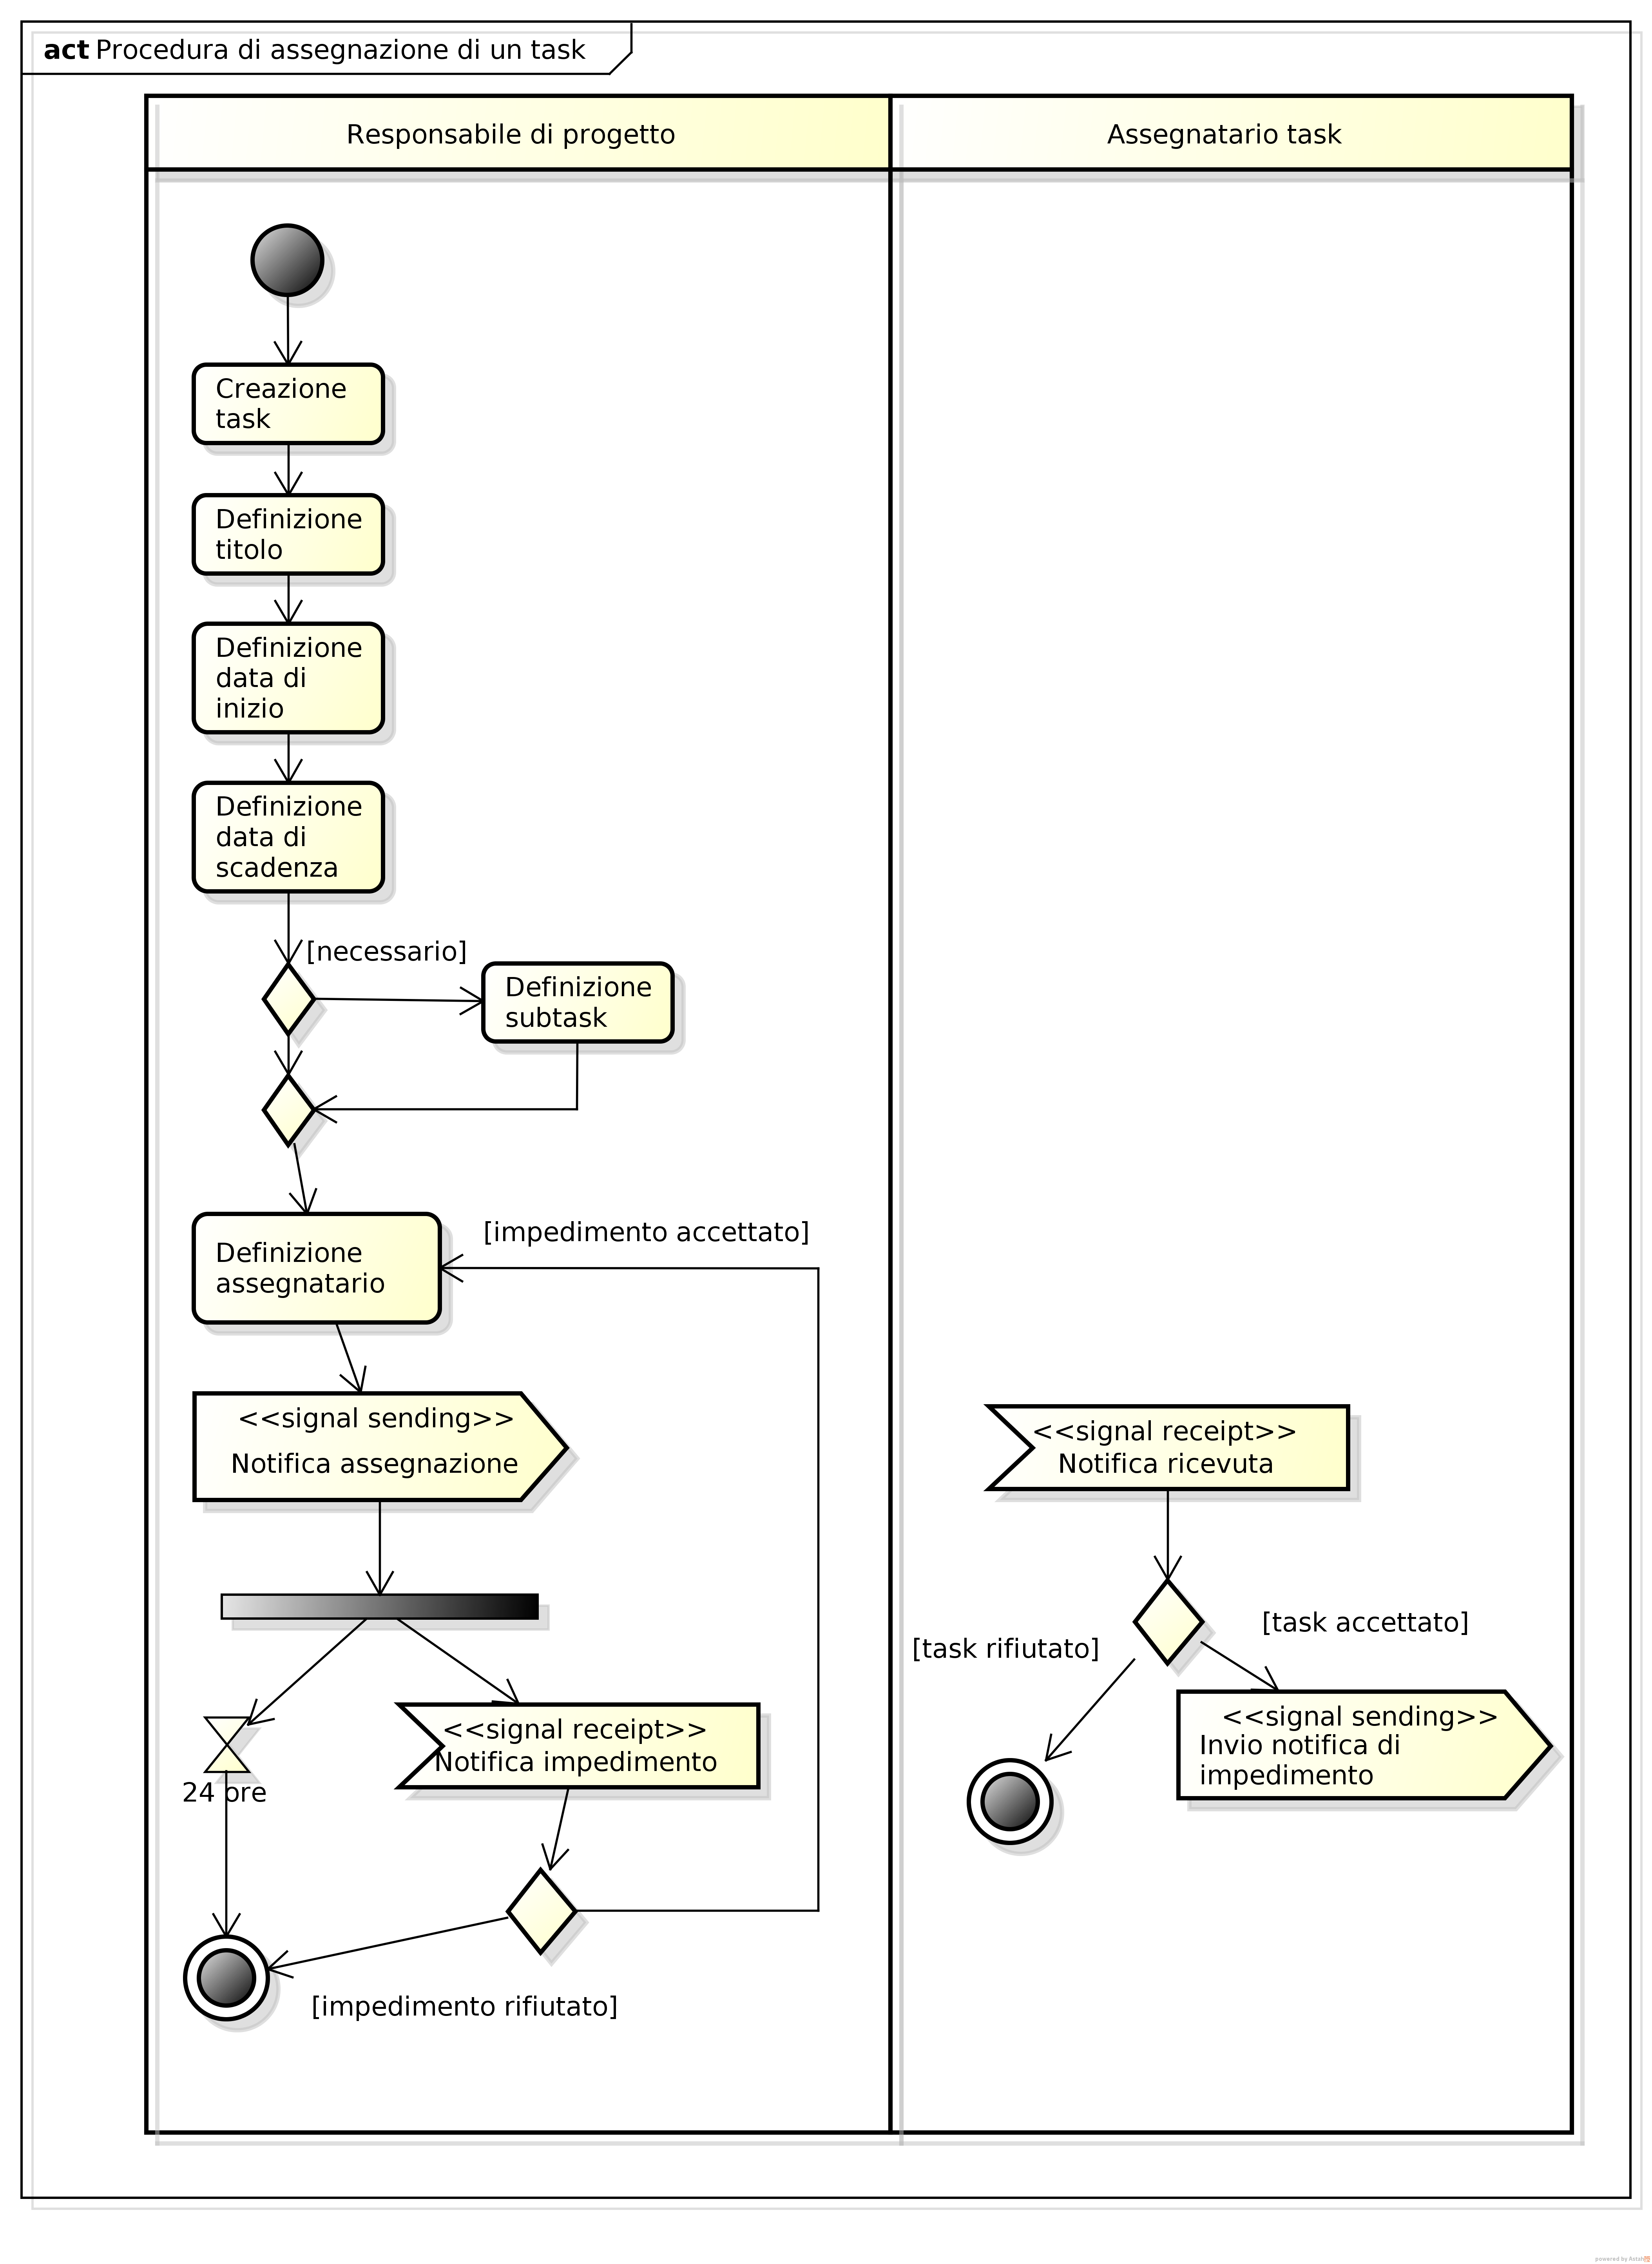
\includegraphics[scale=0.5]{immagini/procedura_di_assegnazione_di_un_task.png}
\captionsetup{labelfont=bf}
\caption{Diagramma di attività - Procedura di assegnazione di un task}\label{sec:Figura6}
\end{figure}

\paragraph{Svolgimento di un task}
Il membro assegnatario del \textit{task}\G, ricevuta la notifica e non avendo alcun impedimento, deve procedere secondo le seguenti direttive, mostrate anche in \hyperref[sec:Figura7]{Figura 7}:
\begin{itemize}
\item [1.] Se il \textit{task} ricevuto ha una scadenza più immediata rispetto a quello su cui sta lavorando, deve sospendere lo svolgimento di quest'ultimo, metterlo in coda e dedicarsi al \textit{task} appena notificato;
\item [2.] Se, dopo aver iniziato lo svolgimento del \textit{task}, si riceve la notifica di uno nuovo con scadenza più immediata si procede come riportato nel punto precedente;
\item [3.] Se si dovesse superare la data di scadenza prevista, è necessario impostare il \textit{tag}\G\ "\textit{Delay}" dal sistema offerto su Teamwork\G. Questa situazione si può verificare se:
\begin{itemize}
\item [-] Il tempo assegnato dal \textit{Responsabile di progetto} non è sufficiente al completamento del \textit{task};
\item [-] Il \textit{task} in ritardo sta alle dipendenze di un altro \textit{task} non ancora completato;
\item [-] L'assegnatario è rallentato da cause esterne non rese note al \textit{Responsabile di Progetto};
\item [-] Il membro incaricato non ha a disposizione tutte le conoscenze necessarie per un corretto svolgimento del \textit{task}.
\end{itemize}
Spetta al \textit{Responsabile di Progetto} fare in modo che i primi due casi non si verifichino.

\item [4.] Al completamento del lavoro l'assegnatario deve spuntare il \textit{task} dalla lista presente su Teamwork\G;
\item [5.] A questo punto può proseguire con lo svolgimento dei \textit{task} rimanenti riprendendo la procedura dall'inizio.
\end{itemize}

\begin{figure}[htbp]
\centering
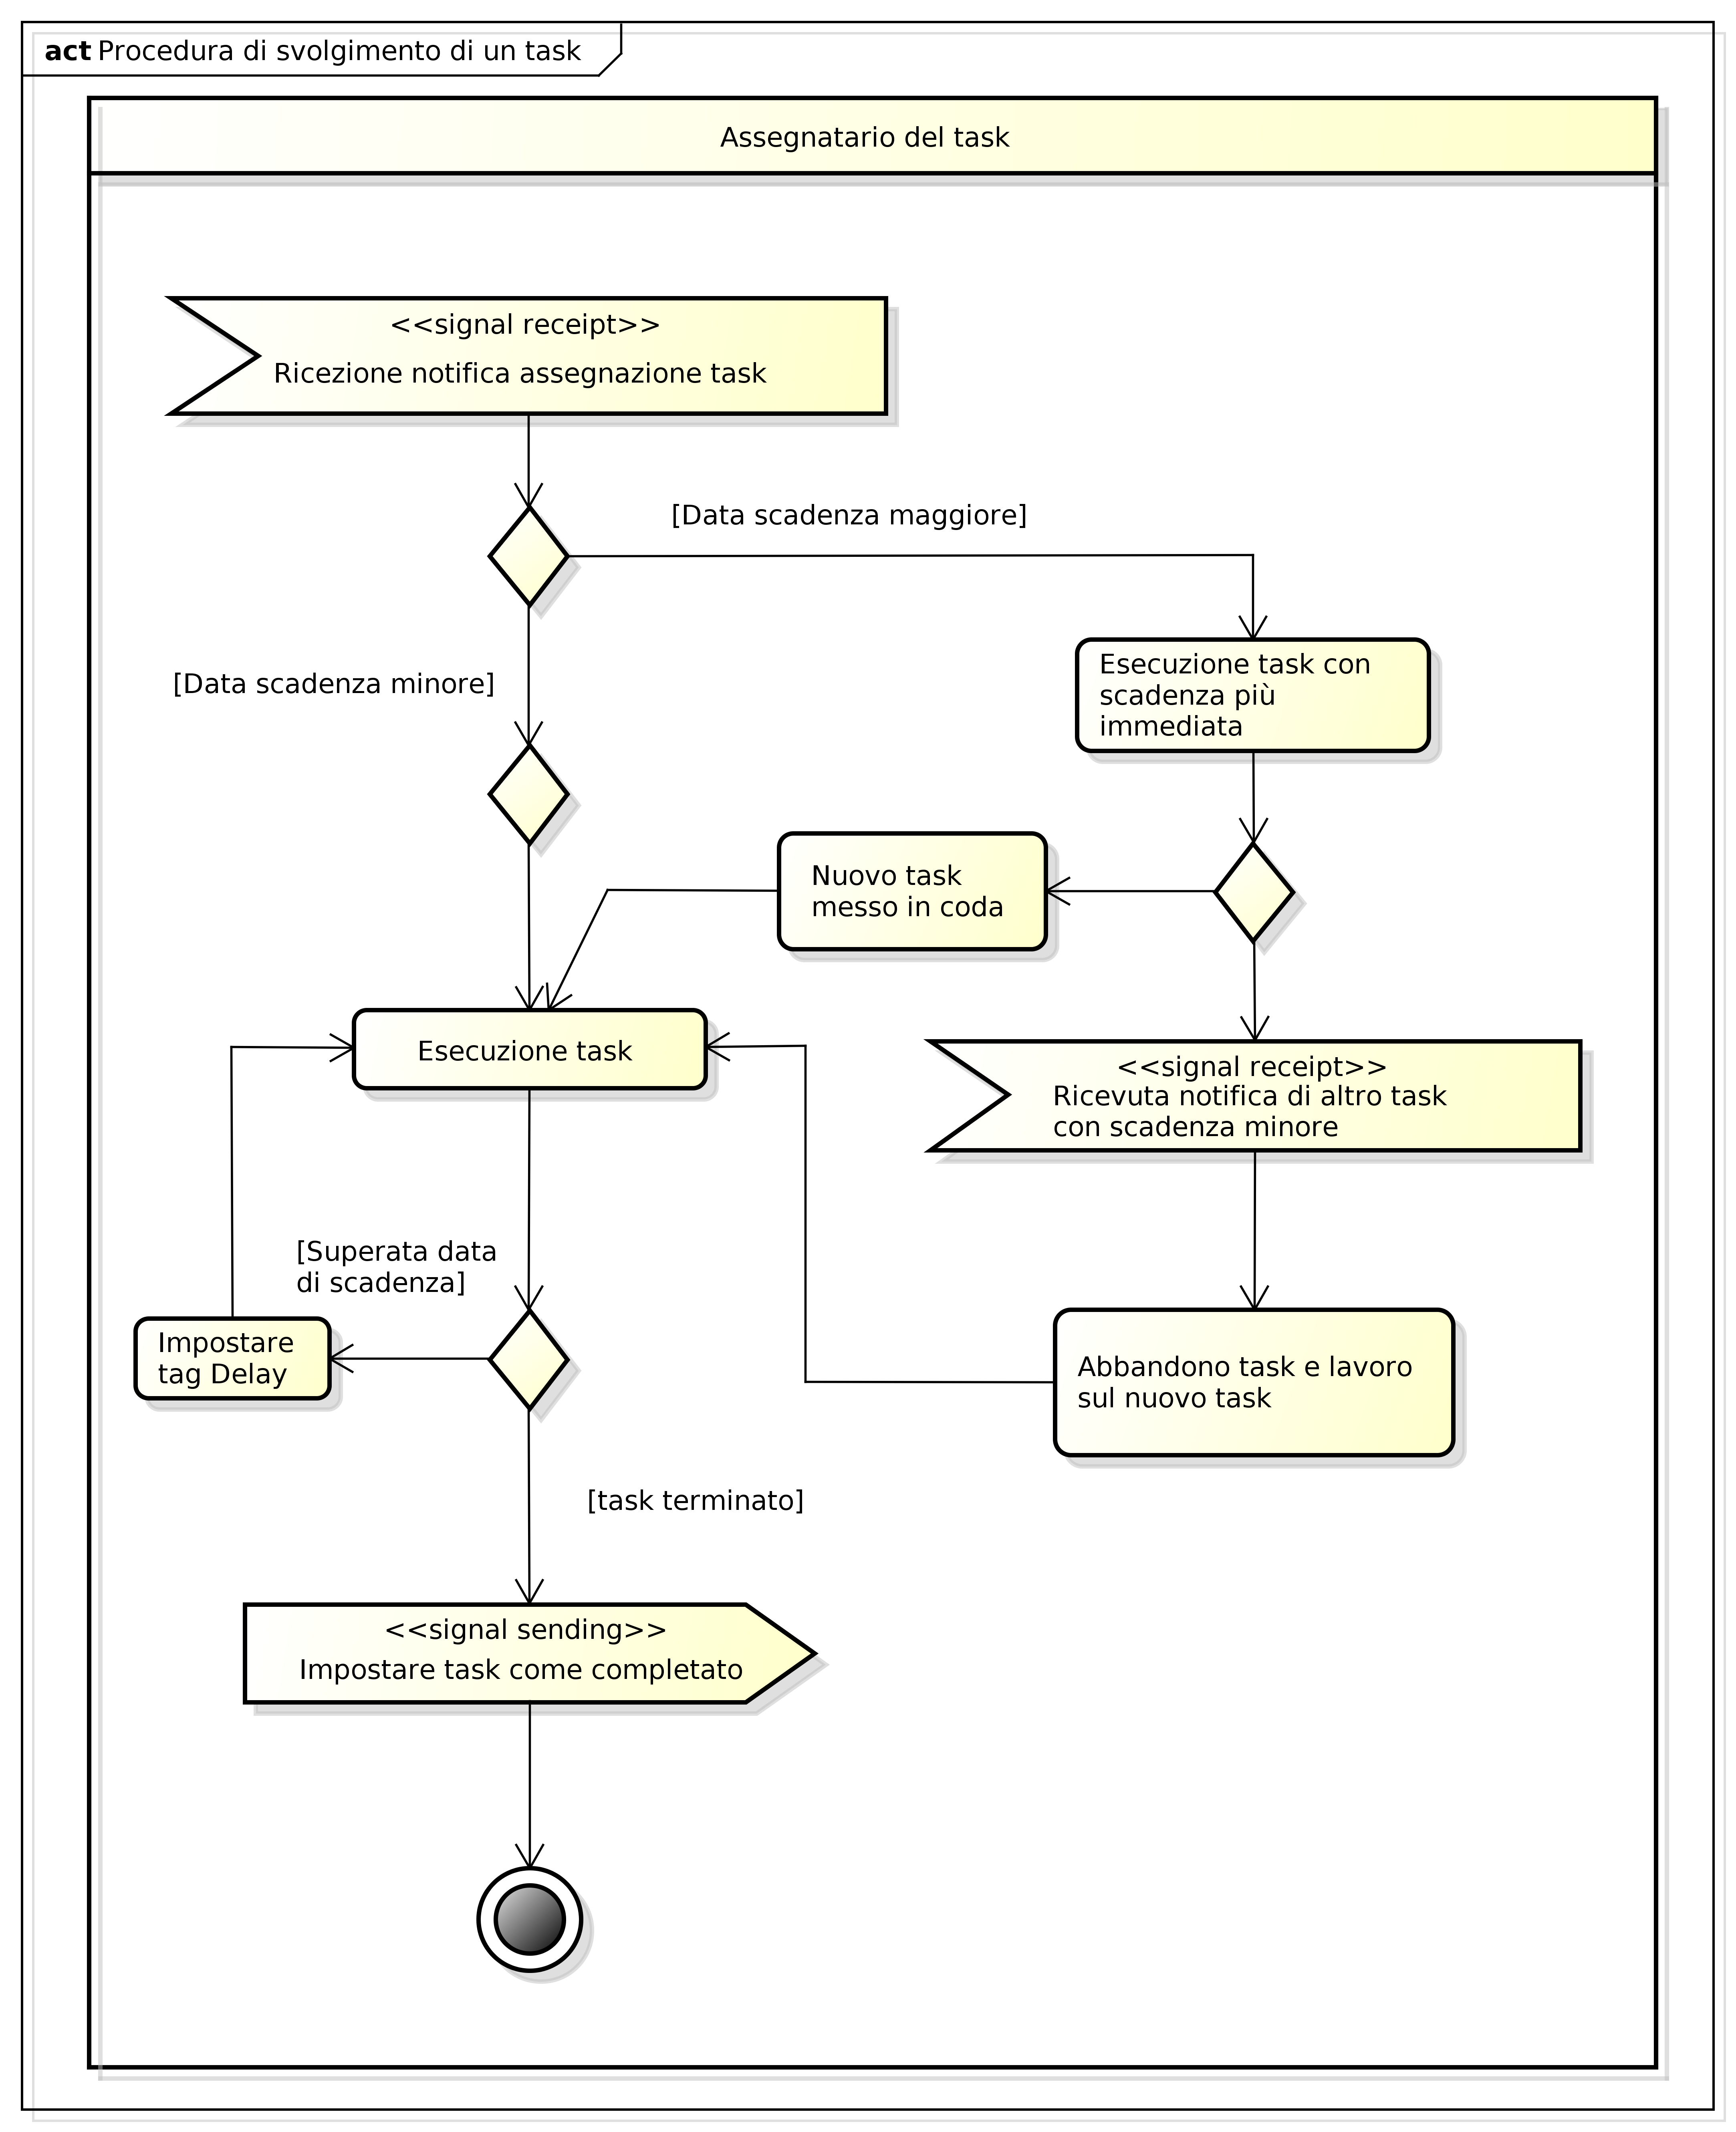
\includegraphics[scale=0.5]{immagini/procedura_di svolgimento_di_un_task.png}
\captionsetup{labelfont=bf}
\caption{Diagramma di attività - Procedura di svolgimento di un task}\label{sec:Figura7}
\end{figure}

\paragraph{Rilevamento dei rischi}
È compito del \textit{Responsabile di Progetto} individuare i rischi trovati nel \textit{Piano di Progetto v1.0.0}. Questa attività necessita di un continuo monitoraggio, in quanto è plausibile che insorgano nuovi rischi in seguito a quelli rilevati nella fase preliminare. In tal caso il \textit{Responsabile di Progetto} deve agire come segue:
\begin{itemize}
\item [1.] Registrare il resoconto effettivo dei rischi nel \textit{Piano di Progetto v1.0.0};
\item [2.] Pianificare per gestire i nuovo rischi;
\item [3.] Aggiornare le metodologie per far fronte alla nuova pianificazione;
\item [4.] Monitorare i nuovo rischi riscontrati durante lo sviluppo del progetto. 
\end{itemize}

\subsubsection{Norme}
\paragraph{Ruoli di Progetto}
Ogni componente del gruppo \GRUPPO\ deve ricoprire almeno una volta ciascuno dei ruoli necessari allo sviluppo del progetto. Nell'assegnazione dei compiti il \textit{team} si impegna a distribuire equamente le ore di lavoro previste per ogni ruolo. Questo criterio ha guidato la stesura del \textit{Piano di Progetto v1.0.0} di cui si rimanda alla lettura.\\
Di seguito vengono presentati i diversi incarichi, delineando per ciascuno mansioni e responsabilità.

\subparagraph{Responsabile di Progetto} Il \textit{Responsabile di Progetto} rappresenta il \textit{team} e il progetto nei confronti di Committente e Proponente; accentra le responsabilità di scelta e approvazione. Detiene inoltre le seguenti responsabilità:
\begin{itemize}
\item Pianificazione e coordinamento delle attività;
\item Gestione e controllo delle risorse;
\item Analisi e gestione dei rischi;
\item Approvazione dei documenti;
\item Assicurarsi che tutte le attività svolte siano conformi alle \textit{Norme di Progetto
v1.0.0} e rispettino la pianificazione effettuata nel \textit{Piano di Progetto v1.0.0}.
\end{itemize}  

\subparagraph{Amministratore di Progetto} L' \textit{Amministratore di Progetto} deve svolgere i seguenti compiti:
\begin{itemize}
\item Assicurarsi che tutte le risorse siano presenti e operanti; 
\item Garantire un'infrastruttura funzionale;
\item Fornire procedure che servono a garantire la qualità del prodotto uscente da un
determinato compito.
\end{itemize}

\subparagraph{Analista} L' \textit{Analista} deve svolgere i seguenti compiti:
\begin{itemize}
\item Tradurre il bisogno del cliente in una specifica utile per trovare una soluzione;
\item Comprendere la complessità del problema;
\item Capire il dominio nel quale lavora il cliente;
\item Analizzare il dominio applicativo e le specifiche per poi produrre i documenti di analisi.
\end{itemize}

\subparagraph{Progettista} Il \textit{Progettista} deve svolgere i seguenti compiti:
\begin{itemize}
\item Individuare la tecnologia più idonea per risolvere il problema indicato dall'\textit{Analista};
\item Descrivere il funzionamento interno del sistema a diversi livelli di dettaglio;
\item Produrre una soluzione comprensibile e attuabile. 
\end{itemize}

\subparagraph{Programmatore} Il \textit{Programmatore} ha responsabilità sulle attività di codifica e pertanto deve svolgere i seguenti compiti:
\begin{itemize}
\item Scrivere codice documentato, versionato e manutenibile;
\item Implementare le soluzioni descritte dal \textit{Progettista};
\item Implementare i \textit{test} sul codice prodotto. 
\end{itemize}

\subparagraph{Verificatore} Il \textit{Verificatore} è il responsabile delle attività di verifica e pertanto deve svolgere i seguenti compiti:
\begin{itemize}
\item Controllare che vengano rispettate le norme di progetto;
\item Assicurarsi la conformità di ogni stadio del ciclo di vita\G\ del prodotto.
\end{itemize}

\subsubsection{Strumenti}

\paragraph{TeXstudio} TeXstudio\G\ è l'\textit{editor} di testo multipiattaforma \textit{open-source}\G\ utilizzato per scrivere documenti in \LaTeX.
\paragraph{Teamwork} Teamwork\G\ è l'applicazione \textit{web} scelta per la gestione dei \textit{task}\G; permette anche di gestire un calendario dove inserire note o fissare appuntamenti e/o traguardi importanti.
\paragraph{Astah} Astah\G\ è l'applicativo scelto per la creazione di grafici UML\G. La versione adottata è quella \textit{Professional}, resa disponibile gratuitamente per un utilizzo da parte di studenti.
\paragraph{Microsoft Project 2016} Microsoft Project 2016 è il \textit{software} utilizzato per la creazione dei grafici di Gantt\G. Si utilizza il contratto Microsoft MSDN-AA (\textit{Academic Alliance}) reso disponibile dal Dipartimento di Matematica dell'Università degli Studi di Padova in accordo con Microsoft.
\paragraph{Telegram} Si utilizza Telegram\G\ per una comunicazione informale all'interno del 
gruppo. Inoltre Telegram fornisce il vantaggio di essere un'applicazione 
multipiattaforma\G\ disponibile nelle seguenti versioni: \textit{desktop}, \textit{web} e \textit{mobile}.
\paragraph{Microsoft Office PowerPoint} PowerPoint\G\ è il software utilizzato per creare presentazioni.

\subsection{Gestione delle infrastrutture}

\paragraph{Attività} 
\subparagraph{Gestione del repository} Il gruppo ha deciso di utilizzare un repository\G\ utile a svolgere funzioni diverse, ma necessarie, allo sviluppo del sistema finale. Una volta iscritto, ciascun membro ha la possibilità di creare il suo \textit{branch}\G\ personale contenente una copia dei file originali del \textit{branch} \textit{master} in modo da poter lavorare su delle copie in locale.

\subparagraph{Gestione del messaggio di commit} Per mantenere l'ambiente di lavoro il meno ambiguo possibile, è stato deciso di adottare un formato standard per andare a scrivere il messaggio della \textit{commit}\G.

\paragraph{Procedure} 
\subparagraph{Installazione di Git} La procedura di installazione varia a seconda del sistema operativo utilizzato. Per i sistemi Linux\G\ occorre rispettare la seguente procedura:
\begin{itemize}
\item Aprire il terminale;
\item Immettere il comando \textit{sudo apt-get update};
\item Immettere il comando \textit{apt-get install git}.
\end{itemize}
Per sistemi OS X\G:
\begin{itemize}
\item Recarsi nella sezione dedicata ai \textit{download} \url{https://git-scm.com/download/mac};
\item Scaricare il \textit{file} in formato DMG\G;
\item Aprire il file appena scaricato;
\item Lanciare l'installazione cliccando su\textit{ git.pkg}.
\end{itemize}
Infine per i sistemi Windows\G, è necessario fare quanto segue:
\begin{itemize}
\item Accedere al sito ufficiale \url{https://git-for-windows.github.io};
\item Scaricare l'eseguibile;
\item Lanciare l'eseguibile;
\item Seguire la procedura riportata dalla finestra di dialogo.
\end{itemize}

\subparagraph{Creazione di una cartella locale di repository} Seguire la seguente procedura:
\begin{itemize}
\item Creare una nuova cartella;
\item Aprire il terminale;
\item Collocarsi all'interno della cartella appena creata;
\item Eseguire il comando \textit{git init}.
\item Immettere il comando \textit{git clone <indirizzo>}, sostituendo <indirizzo> con l'URL del progetto su GitHub\G.
\end{itemize}

\subparagraph{Creazione del branch personale} Per creare il \textit{branch}\G\ personale occorre seguire i seguenti passi:
\begin{itemize}
\item Muoversi nella cartella di \textit{repository}\G.
\item Accedere alla cartella di progetto;
\item Eseguire il comando \textit{git branch <nome>}, sostituendo <nome> con il nome del nuovo \textit{branch} da creare.
\end{itemize}

\subsubsection{Norme}
\paragraph{Repository}
\subparagraph{Nomi dei file in SiVoDiM} I \textit{file} e le cartelle presenti
nel \textit{repository}\G\ devono essere conformi al seguente formalismo tratto dallo Standard
ISO\G\ 9660:1999 (Level 2):
\begin{itemize}
\item I caratteri usati sono solo quelli minuscoli a-z, 0-9, l’\textit{underscore}\G\ e il punto (esempio: nome\_del\_documento.tex);
\item Non sono ammessi caratteri accentati;
\item I nomi non possono includere spazi o finire con un punto (.);
\item I nomi non devono contenere più di un punto (.) utilizzato per separare il nome del \textit{file} dall'estensione (esempio: studio\_di\_fattibilita\_v1\_0\_0.pdf);
\item I nomi non devono essere più lunghi di 21 caratteri esclusi i 3 destinati all’estensione.
\end{itemize}

\subparagraph{Struttura di SiVoDiM}  Le cartelle nel repository\G\ verranno organizzate nel seguente modo a partire dalla \textit{root}\G:
\begin{itemize}
\item \textbf{Documenti}: in essa sono presenti le seguenti cartelle corrispondenti alle varie fasi del processo di sviluppo:
\begin{itemize}
\item \textbf{RR}: contenente i documenti e i file necessari alla revisione dei requisiti;
\item \textbf{RP}: contenente i documenti e i file necessari alla revisione di progettazione;
\item \textbf{RQ}: contenente i documenti e i file necessari alla revisione di qualifica;
\item \textbf{RA}: contenente i documenti e i file necessari alla revisione dei accettazione;
\end{itemize}
\item \textbf{Codice}: la struttura di questa cartella verrà fornita in una fase successiva del lavoro.
\end{itemize}

\subparagraph{Messaggio di commit} Il messaggio di commit\G\ dovrà
essere conforme alla seguente notazione:
\begin{center}
Desc:\\
Data:\\
Note:\\
\end{center}
dove:
\begin{itemize}
\item \textbf{Desc}: fornisce una descrizione esaustiva dell’attività svolta;
\item \textbf{Data}: fornisce la data in cui si è apportata la modifica;
\item \textbf{Note}: aiuta a specificare lo stato del lavoro, nello specifico si adotteranno le seguenti notazioni:
\begin{itemize}
\item [-]{C} se il lavoro è stato completato;
\item [-]{NC} se il lavoro non è stato completato;
\item [-]{V} se il lavoro necessita de verifica;
\end{itemize}
\end{itemize}

\subsubsection{Strumenti}
\paragraph{Git} Git\G\ è il sistema di controllo di versione utilizzato per il \textit{repository}\G\ del \textit{team}.

\paragraph{GitHub} GitHub\G\ è il servizio \textit{web} di \textit{hosting}\G\ adottato per tenere una
copia del \textit{repository}\G\ del progetto.

\paragraph{Dropbox} Dropbox\G\ è lo strumento di \textit{cloud}\G\ che si è scelto
per gestire \textit{file} che non necessitano di essere sottoposti a controllo di versione.

\paragraph{Sistema Operativo} I membri del gruppo operano su tre diversi sistemi operativi:
\begin{itemize}
\item Ubuntu 14.04\G;
\item Linux Mint 17\G;
\item Windows 10\G;
\item OS X 10.11\G.
\end{itemize} 

\subsection{Formazione dei membri del gruppo}
I membri del gruppo che non hanno conoscenze sufficienti per far fronte ai problemi assegnati dal \textit{Responsabile di Progetto}, dovranno
documentarsi e colmare eventuali lacune durante ore esterne a quelle di lavoro, non imputabili perciò ai costi del Committente.



%\input {sections/nomesezione}
%\newpage

% ...

%\printglossaries

\end{document}
